\documentclass[a4paper]{article}
\title{How to Use Player/Stage}
\author{Jennifer Owen}

\usepackage{xspace}
\usepackage{graphicx}
\usepackage{verbatim}
\usepackage{url}

\newcommand{\plst}{Player/Stage\xspace}
\newcommand{\pl}{Player\xspace}


\begin{document}

\maketitle

This document is intended as a guide for anyone learning \plst for the first time. It explains the process of setting up a new simulation environment and how to then make your simulation do something, using a case study along the way. Whilst it is aimed at \plst users, those just wishing to use \pl on their robot may also find sections of this document useful (particularly the parts about coding with Player).

If you have any questions about using \plst there is a guide to getting help from the \pl comunity here:
\begin{center}
	\url{http://playerstage.sourceforge.net/wiki/Getting_help}
\end{center}

\newpage
\tableofcontents

\newpage
\section{Introduction}
\plst is a robot simulation tool, it comprises of one program, \pl, which is a \emph{Hardware Abstraction Layer}. That means that it talks to the bits of hardware on the robot (like a claw or a camera) and lets you control them with your code, meaning you don't need to worry about how the various parts of the robot work. Stage is a plugin to \pl which listens to what \pl is telling it to do and turns these instructions into a simulation of your robot. It also simulates sensor data and sends this to \pl which in turn makes the sensor data available to your code.

A simulation then, is composed of three parts:
\begin{itemize}
\item Your code. This talks to \pl.
\item \pl. This takes your code and sends instructions to a robot. From the robot it gets sensor data and sends it to your code.
\item Stage. Stage interfaces with \pl in the same way as a robot's hardware would. It receives instructions from \pl and moves a simulated robot in a simulated world, it gets sensor data from the robot in the simulation and sends this to \pl.
\end{itemize}
Together \pl and Stage are called \plst, and they make a simulation of your robots.

These instructions will be focussing on how to use \plst to make a simulation, but hopefully this will still be a useful resource for anyone just using \pl (which is the same thing but on a real robot, without any simulation software).

\subsection{A Note on Installing \plst}
Instructions on how to install \plst onto your computer aren't really the focus of this document. It is very difficult though. If you're lucky the install will work first time but there are a lot of dependencies which may need installing. In Linux there are the install programmes ``synaptic'' or ``aptitude'' which will install a package and also get its dependencies, but these aren't common to all Linux distributions. There is another install program called ``apt-get'' but this won't install dependencies for you. For computers running Ubuntu there is a reasonable set of instructions here:
\begin{center}
\url{http://www.control.aau.dk/~tb/wiki/index.php/Installing_Player_and_Stage_in_Ubuntu}
\end{center}
Alternatively, you try the suggestions on the \pl ``getting help'' page:
\begin{center}
	\url{http://playerstage.sourceforge.net/wiki/Getting_help}
\end{center}

\section{The Basics}

\subsection{Important File Types}
In \plst there are 3 kinds of file that you need to understand to get going with \plst:
\begin{itemize}
	\item a .world file
	\item a .cfg (configuration) file
	\item a .inc (include) file
\end{itemize}
The .world file tells \plst what things are available to put in the world. In this file you describe your robot, any items which populate the world and the layout of the world. The .inc file follows the same syntax and format of a .world file but it can be \emph{included}. So if there is an object in your world that you might want to use in other worlds, such as a model of a robot, putting the robot description in a .inc file just makes it easier to copy over, it also means that if you ever want to change your robot description then you only need to do it in one place and your multiple simulations are changed too.

The .cfg file is what \pl reads to get all the information about the robot that you are going to use.This file tells \pl which drivers it needs to use in order to interact with the robot, if you're using a real robot these drivers are built in to \pl\footnote{Or you can download or write your own drivers, but I'm not going to talk about how to do this here.}, alternatively, if you want to make a simulation, the driver is always Stage (this is how \pl uses Stage in the same way it uses a robot: it thinks that it is a hardware driver and communicates with it as such). The .cfg file tells \pl how to talk to the driver, and how to interpret any data from the driver so that it can be presented to your code. Items described in the .world file should be described in the .cfg file if you want your code to be able to interact with that item (such as a robot), if you don't need your code to interact with the item then this isn't necessary. The .cfg file does all this specification using interfaces and drivers, which will be discussed in the following section.

\subsection{Interfaces, Drivers and Devices} \label{sec:interfaceDriverDevices}
\begin{itemize}
\item Drivers are pieces of code that talk directly to hardware. These are built in to \pl so it is not important to know how to write these as you begin to learn \plst. The drivers are specific to a piece of hardware so, say, a laser driver will be different to a camera driver, and also different to a driver for a different brand of laser. This is the same as the way that drivers for graphics cards differ for each make and model of card. Drivers produce and read information which conforms to an ``interface''.

\item Interfaces are a set way for a driver to send and receive information from \pl. Like drivers, interfaces are also built in to \pl and there is a big list of them in the \pl manual\footnote{http://playerstage.sourceforge.net/doc/\pl-2.1.0/player/group\_\_interfaces.html}. They specify the syntax and semantics of how drivers and \pl interact.
	
\item A device is a driver that is bound to an interface so that \pl can talk to it directly. This means that if you are working on a real robot that you can interact with a real device (laser, gripper, camera etc) on the real robot, in a simulated robot you can interact with their simulations. 
\end{itemize}

The official documentation actually describes these 3 things quite well with an example.

\begin{quotation}
	Consider the laser interface. This interface defines a format in which a planar range-sensor can return range readings (basically a list of ranges, with some meta-data). The laser interface is just that: an interface. You can't do anything with it.

	Now consider the sicklms200 driver. This driver controls a SICK LMS200, which is particular planar range sensor that is popular in mobile robot applications. The sicklms200 driver knows how to communicate with the SICK LMS200 over a serial line and retrieve range data from it. But you don't want to access the range data in some SICK-specific format. So the driver also knows how to translate the retrieved data to make it conform to the format defined by the laser interface.

	The sicklms200 driver can be bound to the laser interface \ldots to create a device, which might have the following address:

	localhost:6665:laser:0 \label{sec:setting_a_device}

	The fields in this address correspond to the entries in the \mbox{player\_devaddr\_t} structure: host, robot, interface, and index. The host and robot fields (localhost and 6665) indicate where the device is located. The interface field indicates which interface the device supports, and thus how it can be used. Because you might have more than one laser, the index field allows you to pick among the devices that support the given interface and are located on the given host:robot Other lasers on the same host:robot would be assigned different indexes.
\end{quotation}
The last paragraph there gets a bit technical, but don't worry. \pl talks to parts of the robot using ports (the default port is 6665), if you're using Stage then \pl and Stage communicate through these ports (even if they're running on the same computer). All this line does is tell \pl which port to listen to and what kind of data to expect. In the example it's laser data which is being transmitted on port 6665 of the computer that \pl is running on (localhost). You could just as easily connect to another computer by using its IP address instead of ``localhost''. The specifics of writing a device address in this way will be described in section \ref{sec:WritingConfigurationFile}.

\section{Building a World} \label{sec:BuildingAWorld}

First we will run a world and configuration file that comes bundled with Stage. In your bash shell navigate to the Stage/worlds folder, by default (in Linux at least) this is /usr/local/share/stage/worlds. Once in the correct folder type the following command to run the ``simple world'' that comes with \plst:
\begin{verbatim}
player simple.cfg
\end{verbatim}
Assuming \plst is installed properly you should now have a window open which looks figure \ref{fig:simpleworldpic}.
\begin{figure}
	\centering
	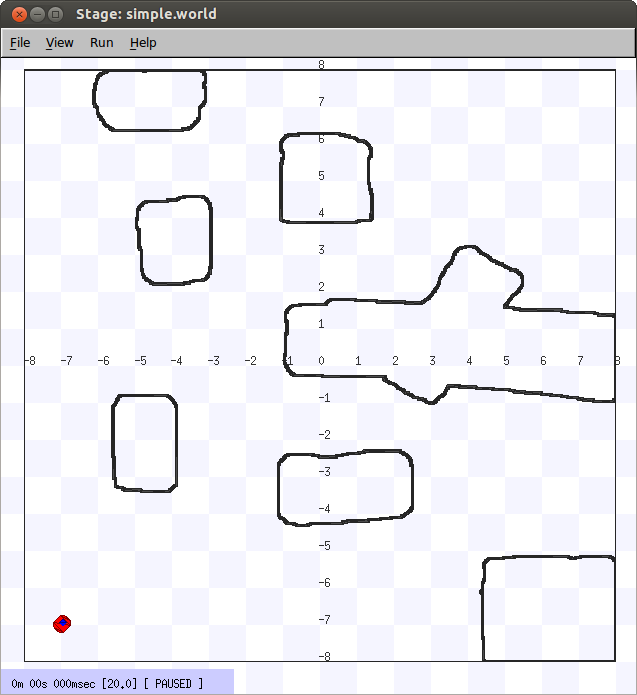
\includegraphics[width=0.8\linewidth]{./pics/simpleworld.png}
	\caption{The simple.cfg world after being run}
	\label{fig:simpleworldpic}
\end{figure}
At this stage you can drag and drop the robot around its world with your mouse, but you can also tele-operate the robot using the \pl Viewer program. In a \emph{separate terminal} whilst the \plst simulation window is still open, type:
\begin{verbatim}
playerv --position2d --laser
\end{verbatim}
The \verb|--position2d| and \verb|--laser| options tell the playerv (\pl Viewer) program that you want to look at the positional data and the laser data that is available to the robot. This should open a window which looks like figure \ref{fig:playerv_simpleworldpic}. 

To be able to remote control the robot you click Device $\rightarrow$ position2d:0 $\rightarrow$ Command as shown in figure \ref{fig:playerv_teleoperation}. A cross-hair should appear over the robot in the \pl Viewer window, which if you drag around will cause the robot to move in the \plst simulation (figure \ref{fig:simpleworldpic}).

\begin{figure}
	\centering
	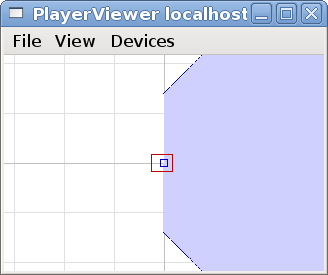
\includegraphics[width=0.4\linewidth]{./pics/playerv_simpleworld.png}
	\caption{The simple.cfg world seen with \pl Viewer}
	\label{fig:playerv_simpleworldpic}
\end{figure}

\begin{figure}
	\centering
	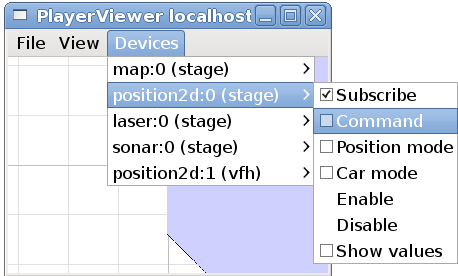
\includegraphics[width=0.6\linewidth]{./pics/playerv_teleoperation.png}
	\caption{How to Remote Control (tele-operate) the Stage Robot}
	\label{fig:playerv_teleoperation}
\end{figure}



\subsection{Building an Empty World} \label{sec:emptyWorld}

As you can see in section \ref{sec:BuildingAWorld}, when we tell \pl to build a world we only give it the .cfg file as an input. This .cfg file needs to tell us where to find our .world file, which is where all the items in the simulation are described. To explain how to build a Stage world containing nothing but walls we will use an example.\newline
To start building an empty world we need a .cfg file. First create a document called \verb|empty.cfg| and copy the following code into it:
\begin{verbatim}
driver
(		
      name "stage"
      plugin "libstageplugin"

      provides ["simulation:0" ]

      # load the named file into the simulator
      worldfile "empty.world"	
)
\end{verbatim}
The configuration file syntax is described in section \ref{sec:WritingConfigurationFile}, but basically what is happening here is that your configuration file is telling \pl that there is a driver called \verb|stage| in the \verb|libstageplugin| library, and this will give \pl data which conforms to the \verb|simulation| interface. To build the simulation \pl needs to look in the worldfile called \verb|empty.world| which is stored in the same folder as this .cfg. If it was stored elsewhere you would have to include a filepath, for example \verb|./worlds/empty.world|. Lines that begin with the hash symbol (\#) are comments.
When you build a simulation, any simulation, in Stage the above chunk of code should always be the first thing the configuration file says. Obviously the name of the worldfile should be changed depending on what you called it though.

Now a basic configuration file has been written, it is time to tell \plst what to put into this simulation. This is done in the .world file. 

\subsubsection{Models} \label{sec:models}
A worldfile is basically just a list of models that describes all the stuff in the simulation. This includes the basic environment, robots and other objects. The basic type of model is called ``model'', and you define a model using the following syntax:
\begin{verbatim}
define model_name model
(
      # parameters
)
\end{verbatim}
This tells \plst that you are \verb|defining| a \verb|model| which you have called \verb|model_name|, and all the stuff in the round brackets are parameters of the model. To begin to understand \plst model parameters, let's look at the \verb|map.inc| file that comes with Stage, this is used to describe the basic environment in the simulation (e.g. walls the robots can bump into):
\begin{verbatim}
define map model
(
  # sombre, sensible, artistic
  color "black"

  # most maps will need a bounding box
  boundary 1

  gui_nose 1
  gui_grid 1
  gui_movemask 0
  gui_outline 0
 
  fiducial_return 0
  gripper_return 0
)
\end{verbatim}
We can see from the first line that they are defining a \verb|model| called \verb|map|. 
\begin{itemize}
\item \verb|color|: Tells \plst what colour to render this model, in this case it is going to be black. 
\item boundary: Whether or not there is a bounding box around the model. This is an example of a binary parameter, which means the if the number next to it is 0 then it is false, if it is 1 or over then it's true. So here we DO have a bounding box around our ``map'' model so the robot can't wander out of our map.
\item \verb|gui_nose|: this tells \plst that it should indicate which way the model is facing. Figure \ref{fig:guinose} shows the difference between a map with a nose and one without.
\item \verb|gui_grid|: this will superimpose a grid over the model. Figure \ref{fig:guigrid} shows a map with a grid.
\item \verb|gui_movemask|: this indicates whether it should be possible to drag and drop the model. Here it is 0, so you cannot move the map model once \plst has been run. In section \ref{sec:BuildingAWorld} when the \plst example \verb|simple.cfg| was run it was possible to drag and drop the robot because its \verb|gui_movemask| variable was set to 1.
\item \verb|gui_outline|: indicates whether or not the model should be outlined. This makes no difference to a map, but it can be useful when making models of items within the world.


\item \verb|fiducial_return|: any parameter of the form some\_sensor\_return describes how that kind of sensor should react to the model. ``Fiducial'' is a kind of robot sensor which will be described later in section \ref{sec:robotSensors}. Setting \verb|fiducial_return| to 0 means that the map cannot be detected by a fiducial sensor.
\item \verb|gripper_return|: Like \verb|fiducial_return|, \verb|gripper_return| tells \plst that your model can be detected by the relevant sensor, ie it can be gripped by a gripper. This parameter also indicates whether the model can be pushed. Here \verb|gripper_return| is set to 0 so the map cannot be pushed by a robot and it cannot be gripped by a gripper.
\end{itemize}

\begin{figure}
	\centering
	\begin{minipage}[c]{0.45\linewidth}
		\centering
		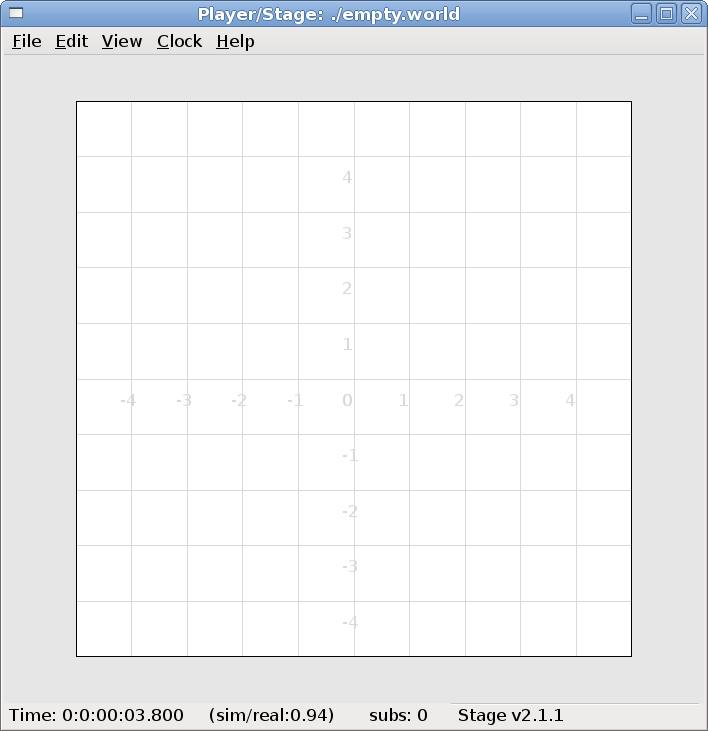
\includegraphics[width=\linewidth]{./pics/emptyWorld/gui_nonose_example.png}
		
	\end{minipage}%
	\hspace{0.05\linewidth}
	\begin{minipage}[c]{0.45\linewidth}
		\centering
		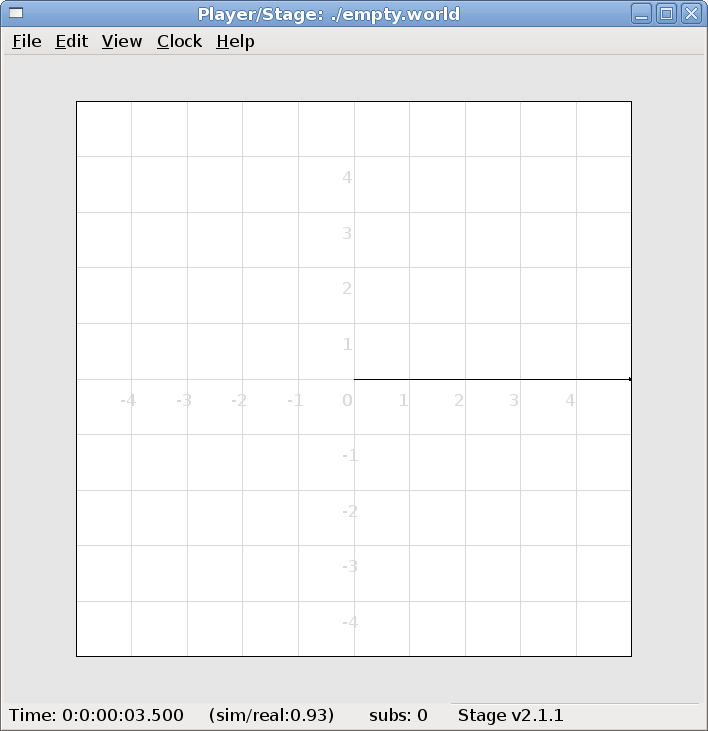
\includegraphics[width=\linewidth]{./pics/emptyWorld/gui_nose_example.png} 
	\end{minipage}	
	\caption{The left picture shows an empty map without a nose. The right picture shows the same map with a nose to indicate orientation, this is the horizontal line from the centre of the map to the right, it shows that the map is actually facing to the right.}
		\label{fig:guinose}
\end{figure}

\begin{figure}
	\centering
	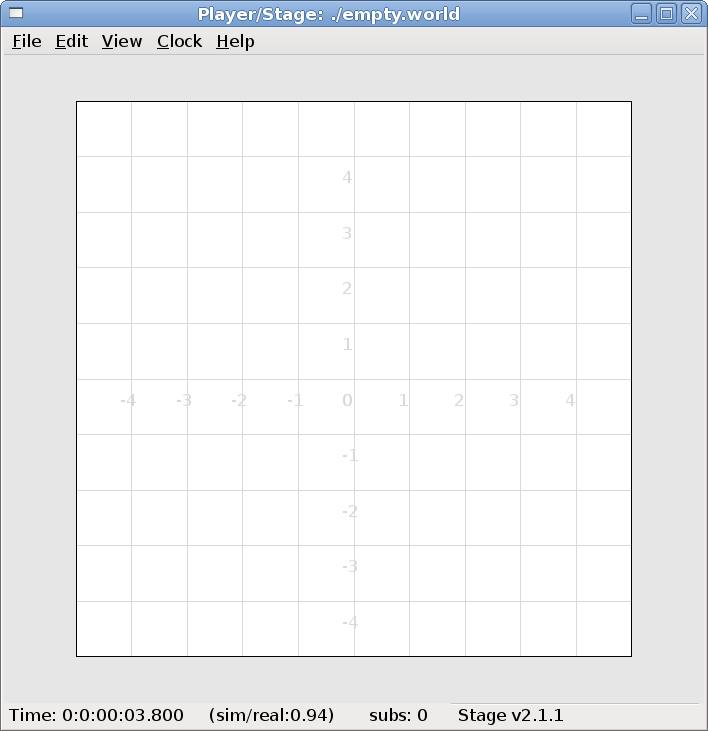
\includegraphics[width=0.7\linewidth]{./pics/emptyWorld/gui_nonose_example.png}
	\caption{An empty map with gui\_grid enabled. With gui\_grid disabled this would just be an empty white square.}
	\label{fig:guigrid}
\end{figure}

To make use of the \verb|map.inc| file we put the following code into our world file:
\begin{verbatim}
include "map.inc"
\end{verbatim}
This inserts the \verb|map.inc| file into our world file where the include line is. This assumes that your worldfile and \verb|map.inc| file are in the same folder, if they are not then you'll need to include the filepath in the quotes. Once this is done we can modify our definition of the map model to be used in the simulation. For example:
\begin{verbatim}
map
(
      bitmap "bitmaps/helloworld.png"
      size [12 5]	
)
\end{verbatim}
What this means is that we are using the model ``map'', and making some extra definitions; both ``bitmap'' and ``size'' are parameters of a \plst model. Here we are telling \plst that we defined a bunch of parameters for a type of model called ``map'' (contained in map.inc) and now we're using this ``map'' model definition and adding a few extra parameters.
\begin{itemize}
\item \verb|bitmap|: this is the filepath to a bitmap, which can be type bmp, jpeg, gif or png. Black areas in the bitmap tell the model what shape to be, non-black areas are not rendered, this is illustrated in figure \ref{fig:helloWorldBitmap}. In the map.inc file we told the map that its ``color'' would be black. This parameter does not affect how the bitmaps are read, \plst will always look for black in the bitmap, the ``color'' parameter just alters what colour the map is rendered in the simulation. 
\item \verb|size|: This is the size \emph{in metres} of the simulation. All sizes you give in the world file are in metres, and they represent the actual size of things. If you have 3m x 4m robot testing arena which you want to simulate then the size here is [3.0 4.0]. The first number is the size in the $x$ dimension, the second is the $y$ dimension.
\end{itemize}

\begin{figure}
	\centering
	\begin{minipage}[c]{0.4\linewidth}
		\centering
		
\includegraphics[width=\linewidth]{./pics/emptyWorld/writing.png}
		
	\end{minipage}%
	\hspace{0.05\linewidth}
	\begin{minipage}[c]{0.5\linewidth}
		\centering
		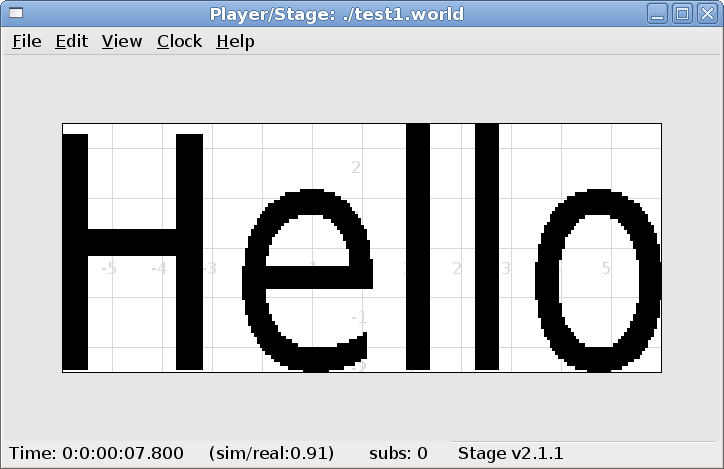
\includegraphics[width=\linewidth]{./pics/emptyWorld/bitmapHello.png} 
	\end{minipage}	
	\caption{The left image is our "helloworld.png" bitmap, the right image is what \plst interprets that bitmap as. The black areas are walls, the robot can move everywhere else.}
		\label{fig:helloWorldBitmap}
\end{figure}

A full list of model parameters and their descriptions can be found in the official Stage manual\footnote{http://playerstage.sourceforge.net/doc/stage-3.0.1/group\_\_model.html}. Most of the useful parameters have already been described here, however there are a few other types of model which are relevant to building simulations of robots, these will be described later in section \ref{sec:buildingRobot}.


\subsubsection{Describing the \plst Window}

The worldfile also can be used to describe the simulation window that \plst creates. \plst will automatically make a window for the simulation if you don't put any window details in the worldfile, however, it is often useful to put this information in anyway. This prevents a large simulation from being too big for the window, or to increase or decrease the size of the simulation.

Like a model, a window is an inbuilt, high-level entity with lots of parameters. Unlike models though, there can be only one window in a simulation and only a few of its parameters are really needed. The simulation window is described with the following syntax:
\begin{verbatim}
window
(
      parameters...
)
\end{verbatim}

The two most important parameters for the window are \verb|size| and \verb|scale|.
\begin{itemize}
\item \verb|size|: This is the size the simulation window will be \emph{in pixels}. You need to define both the width and height of the window using the following syntax: \verb|size [width height]|. 
\item \verb|scale|: This is how many metres of the simulated environment each pixel shows. The bigger this number is, the smaller the simulation becomes. The optimum value for the scale is $\frac{map\_size}{window\_size}$ and it should be rounded upwards slightly so the simulation is a little smaller than the window it's in. 
\end{itemize}

A full list of window parameters can be found in the Stage manual under ``WorldGUI''\footnote{http://playerstage.sourceforge.net/doc/stage-3.0.1/group\_\_worldgui.html}.

\subsubsection{Making a Basic Worldfile}\label{sec:basicWorldfile}

We have already discussed the basics of worldfile building: models and the window. There are just a few more parameters to describe which don't belong in either a model or a window description which should be defined and then the worldfile can be built.
\begin{itemize}
\item \verb|size|: At this level this represents how big, in metres, the whole simulation environment will be. This is completely separate from the map size because it could be larger and there might be several different maps running in the same simulation (so more than one simulation could be run at once). Generally though this just needs to be the same as the map size. This parameter must be included in the worldfile otherwise the simulation won't work.
\item \verb|interval_sim|: This is how many simulated milliseconds there are between each update of the simulation window, the default is 100 milliseconds.
\item \verb|interval_real|: This is how many real milliseconds there are between each update of the simulation window. Balancing this parameter and the \verb|interval\_sim| parameter controls the speed of the simulation. Again, the default value is 100 milliseconds, both these interval parameter defaults are fairly sensible, so it's not always necessary to redefine them.
\end{itemize}
The Stage manual contains a list of the high-level worldfile parameters\footnote{http://playerstage.sourceforge.net/doc/stage-3.0.1/group\_\_world.html}.\newline
Finally, we are able to write a worldfile!
\begin{verbatim}
include "map.inc"

# size of the whole simulation
size [15 15]


# configure the GUI window
window
( 
      size [ 700.0 700.0 ] 
      # 15/700 rounded up a bit
	  scale 0.025
)


# load an environment bitmap
map
(
      bitmap "bitmaps/cave.png"
      size [15 15]	
)
\end{verbatim}
If we save the above code as empty.world (correcting any filepaths if necessary) we can run its corresponding empty.cfg file (see section \ref{sec:emptyWorld}) to get the simulation shown in figure \ref{fig:finalEmptyWorld}.

\begin{figure}
	\centering
	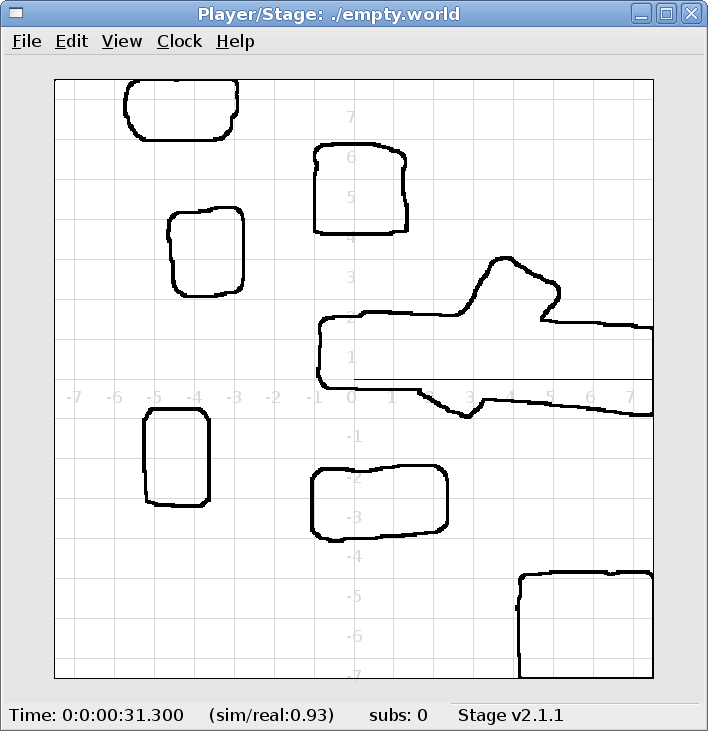
\includegraphics[width=0.7\linewidth]{./pics/emptyWorld/finalEmptyWorld.png} 
	\caption{Our Empty World.}
	\label{fig:finalEmptyWorld}
\end{figure}


\subsection{Building a Robot} \label{sec:buildingRobot}

In \plst a robot is just a slightly advanced kind of model, all the parameters described in section \ref{sec:models} can still be applied. 

\subsubsection{Sensors and Devices} \label{sec:robotSensors}

There are six built-in kinds of model that help with building a robot, they are used to define the sensors and actuators that the robot has. These are associated with a set of model parameters which define by which sensors the model can be detected (these are the \verb\_return\s mentioned earlier). Each of these built in models acts as an \emph{interface} (see section \ref{sec:interfaceDriverDevices}) between the simulation and \pl. If your robot has one of these kinds of sensor on it, then you need to use the relevant model to describe the sensor, otherwise Stage and \pl won't be able to pass the data between each other. It is possible to write your own interfaces, but the stuff already included in \plst should be sufficient for most people's needs. A full list of interfaces that \pl supports can be found in the \pl manual\footnote{http://playerstage.sourceforge.net/doc/\pl-2.1.0/player/group\_\_interfaces.html} although only the following are supported by the current distribution of Stage (version 3.0.1). Unless otherwise stated, these models use the \pl interface that shares its name:

\paragraph{camera}\footnote{http://playerstage.sourceforge.net/doc/stage-3.0.1/group\_\_model\_\_camera.html}
The camera model adds a camera to the robot model and allows your code to interact with the simulated camera. The camera parameters are as follows:
\begin{itemize}
\item \verb|resolution [x y]|: the resolution, in pixels, of the camera's image.
\item \verb|range [min max]|: the minimum and maximum range that the camera can detect
\item \verb|fov [x y]|: the field of view of the camera in degrees.
\item \verb|pantilt [pan tilt]|: the horizontal angle the camera can move through (pan) and the vertical angle (tilt). So for instance \verb\pantilt [90 20]\ allows the camera to move $45^\circ$ left and $45^\circ$ right and $10^\circ$ up and $10^\circ$ down.
\end{itemize}

\paragraph{blobfinder}\footnote{http://playerstage.sourceforge.net/doc/stage-3.0.1/group\_\_model\_\_blobfinder.html}
This simulates colour detection software that can be run on the image from the robot's camera. It is not necessary to include a model of the camera in your description of the robot if you want to use a blobfinder, the blobfinder will work on its own. The blobfinder can only find a model if its \verb|blob_return| parameter is true. The parameters for the blobfinder are described in the Stage manual, but the most useful ones are here:
\begin{itemize}
\item \verb|colors_count <int>|: the number of different colours the blobfinder can detect
\item \verb|colors [ ]|: the names of the colours it can detect. This is given to the blobfinder definition in the form \verb|["black" "blue" "cyan"]|. These colour names are from the built in X11 colour database rgb.txt. This is built in to Linux.\footnote{rgb.txt can normally be found at /usr/share/X11/rgb.txt assuming it's properly installed, alternatively a Google search for ``rgb.txt'' will give you the document.}
\item \verb|image [x y]|: the size of the image from the camera, in pixels.
\item \verb|range <float>|: The maximum range that the camera can detect, in metres.
\item \verb|fov <float>|: field of view of the blobfinder \emph{in RADIANS}.
\end{itemize}
It is important to note that the syntax for the blobfinder model is different in Stage versions 2.X.X and 3.X.X. The above parameters are specific to Stage 3.X.X, in Stage 2.X.X they have different names but do the same thing:
\begin{itemize}
\item \verb|channel_count <int>|: same as colors\_count.
\item \verb|channels [ ]|: same as colors [ ].
\item \verb|image [x y]|: same as in Stage 3.X.X.
\item \verb|range_max <float>|: same as range
\item \verb|ptz [pan_angle tilt_angle zoom_angle]|: controls the areas that the camera can look at. This works like \verb\pantilt\ of the camera model, the \verb\zoom_angle\ is the field of view \emph{in DEGREES}.
\end{itemize}
Additionally, in Stage 2.X.X blobfinder is a child of a deprecated model called ptz. All this basically means is that when you define your blobfinder model you need to use this syntax instead:
\begin{verbatim}
define model_name ptz
(
      blobfinder
      (
            # parameters
      )
)
\end{verbatim}

\paragraph{fiducialfinder}\footnote{http://playerstage.sourceforge.net/doc/stage-3.0.1/group\_\_model\_\_fiducial.html}
A fiducial is a fixed point in an image, so the fiducial finder simulates image processing software that locates fixed points in an image. The fiducialfinder is able to locate objects in the simulation whose \verb|fiducial_return| parameter is set to true. Stage also allows you to specify different types of fiducial using the \verb|fiducial_key| parameter of a model. This means that you can make the robots able to tell the difference between different fiducials by what key they transmit. The fiducial finder and the concept of \verb|fiducial_key|s is properly explained in the Stage manual.

\paragraph{ranger}\footnote{http://playerstage.sourceforge.net/doc/stage-3.0.1/group\_\_model\_\_ranger.html}\label{sec:ranger}
This simulates any kind of obstacle detection device (e.g. sonars or infra-red sensors). These can locate models whose \verb|ranger_return| is true. Using a ranger model you can define any number of ranger devices and apply them all to a single robot. Unlike the other types of model this doesn't use the interface with its name but instead the \verb\sonar\ interface, there is more about this in section \ref{sec:finishConfigs}. The parameters for the \verb\ranger\ model and their inputs are described in the Stage manual, but basically:
\begin{itemize} 
\item \verb|scount <int>|: The number of ranger sensors in this ranger model
\item \verb|spose[ranger_number] [x y yaw]|: Tells the simulator where the rangers are placed around the robot. How to write the \verb|[x y yaw]| data is explained in section \ref{sec:examplerobotsensors}.
\item \verb|ssize [x y]|: how big the sensors are.
\item \verb|sview [min max fov]|: defines the maximum and minimum distances that can be sensed and also the field of view in degrees.
\end{itemize}

\paragraph{laser}\footnote{http://playerstage.sourceforge.net/doc/stage-3.0.1/group\_\_model\_\_laser.html}
A laser is a special case of ranger sensor which only allows one ranger (so there's none of the \verb|scount|, \verb|spose| stuff), but it has a very large field of view. If a model has its \verb|laser_return| parameter enabled then a laser can detect it. Details about laser parameters can be found in the Stage manual, however the most useful parameters are:
\begin{itemize}
\item \verb|range_min|: The minimum range of the laser.
\item \verb|range_max|: the maximum range of the laser.
\item \verb|fov|: the field of view of the laser. In Stage 3.X.X this is in radians, in Stage 2.X.X it is in degrees.
\end{itemize}

\paragraph{gripper}\footnote{http://playerstage.sourceforge.net/doc/Stage-2.0.0/group\_\_model\_\_gripper.html}\label{sec:gripper}
The gripper model is a simulation of the gripper you get on a Pioneer robot.\footnote{The Pioneer grippers looks like a big block on the front of the robot with two big sliders that close around an object.} If you put a gripper on your robot model it means that your robot is able to pick up objects and move them around within the simulation. The online Stage manual says that grippers are deprecated in Stage 3.X.X, however this is not actually the case and grippers are very useful if you want your robot to be able to manipulate and move items. The parameters you can use to customise the gripper model are:
\begin{itemize}
	\item \verb\size [x y]\: The x and y dimensions of the gripper.
	\item \verb\pose [x y yaw]\: Where the gripper is placed on the robot.  
\end{itemize}

\paragraph{position}\footnote{http://playerstage.sourceforge.net/doc/stage-3.0.1/group\_\_model\_\_position.html}\label{sec:position}
The position model simulates the robot's odometry, this is when the robot keeps track of where it is by recording how many times its wheels spin and the angle it turns. This robot model is the most important of all because it allows the robot model to be embodied in the world, meaning it can collide with anything which has its \verb|obstacle_return| parameter set to true. The position model uses the \verb|position2d| interface, which is essential for \pl because it tells \pl where the robot actually is in the world.
The most useful parameters of the position model are:
\begin{itemize}
\item \verb|drive|: Tells the odometry how the robot is driven. This is usually ``diff'' which means the robot is controlled by changing the speeds of the left and right wheels independently. Other possible values are ``car'' which means the robot uses a velocity and a steering angle, or ``omni'' which means it can control how it moves along the $x$ and $y$ axes of the simulation.
\item \verb|localization|: tells the model how it should record the odometry ``odom'' if the robot calculates it as it moves along or ``gps'' for the robot to have perfect knowledge about where it is in the simulation. 
\item \verb|odom_error [x y angle]|: The amount of error that the robot will make in the odometry recordings.
\item \verb|mass <int>|: How heavy the robot is.
\end{itemize}


\subsubsection{An Example Robot} \label{sec:exampleRobot}

To demonstrate how to build a model of a robot in \plst we will build our own example. First we will describe the physical properties of the robot, such as size, shape and mass. Then we will add sensors onto it so that it can interact with its environment.

\paragraph{The Robot's Body}
Let's say we want to model a rubbish collecting robot called ``Bigbob''. The first thing we need to do is describe its basic shape, to do this you need to know your robot's dimensions in metres. Figure \ref{fig:basicbigbob} shows the basic shape of Bigbob drawn onto some cartesian coordinates, the coordinates of the corners of the robot have been recorded. We can then build this model using the \verb|polygons| model parameter\footnote{In this example we're using polygons with the position model type but we could equally use it with other model types.}:
\begin{figure}
	\centering
	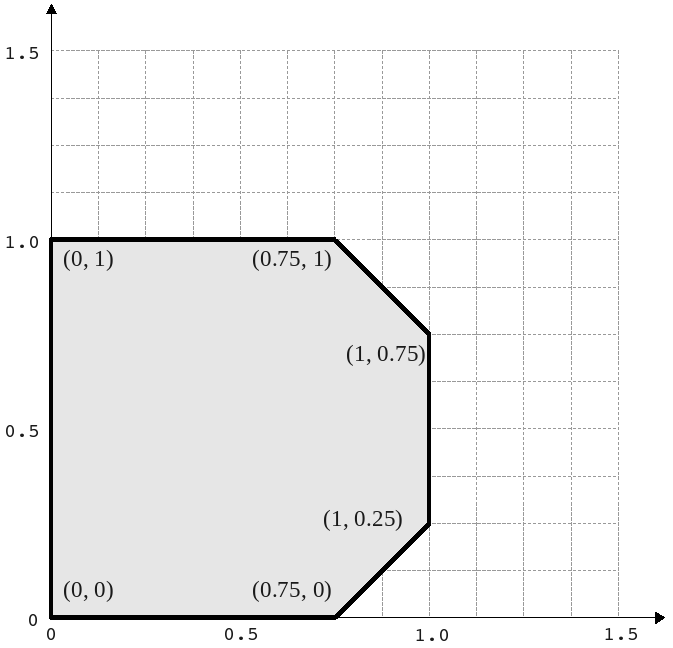
\includegraphics[width=0.7\linewidth]{./pics/robot_building/bigbob1.png} 
	\caption{The basic shape we want to make Bigbob, the units on the axes are in metres.}
	\label{fig:basicbigbob}
\end{figure}

\begin{verbatim}
define bigbob position
(
      # the shape of Bigbob
      polygons 1
      polygon[0].points 6
      polygon[0].point[0] [0 0]
      polygon[0].point[1] [0 1]
      polygon[0].point[2] [0.75 1]
      polygon[0].point[3] [1 0.75]
      polygon[0].point[4] [1 0.25]
      polygon[0].point[5] [0.75 0]
)
\end{verbatim}
In the first line of this code we state that we are defining a \verb|position| model called \verb|bigbob|. Next \verb|polygons 1| says that this model will be built out of one polygon. The following lines go on to describe the shape of this polygon;  \verb|polygon[0].points 6| says that the polygon has 6 corners and \verb|polygon[number].point[number] [x y]| gives the coordinates of each corner of the polygon in turn. It is important to go around the robot doing each corner in turn (either clockwise or anti-clockwise) otherwise \plst won't properly render the polygon. \newline
Now in the same way as we built the body we can add on some teeth for Bigbob to collect rubbish between:
\begin{verbatim}
define bigbob position
(
      # actual size
      size [1.25 1]

      # the shape of Bigbob
      polygons 3
      
      # body
      polygon[0].points 6
      polygon[0].point[0] [0 0]
      polygon[0].point[1] [0 1]
      polygon[0].point[2] [0.75 1]
      polygon[0].point[3] [1 0.75]
      polygon[0].point[4] [1 0.25]
      polygon[0].point[5] [0.75 0]

      # first tooth
      polygon[1].points 4
      polygon[1].point[0] [1 0.75]
      polygon[1].point[1] [1.25 0.75]
      polygon[1].point[2] [1.25 0.625]
      polygon[1].point[3] [1 0.625]

      # second tooth
      polygon[2].points 4
      polygon[2].point[0] [1 0.375]
      polygon[2].point[1] [1.25 0.375]
      polygon[2].point[2] [1.25 0.25]
      polygon[2].point[3] [1 0.25]
)
\end{verbatim}

\begin{figure}
	\centering
	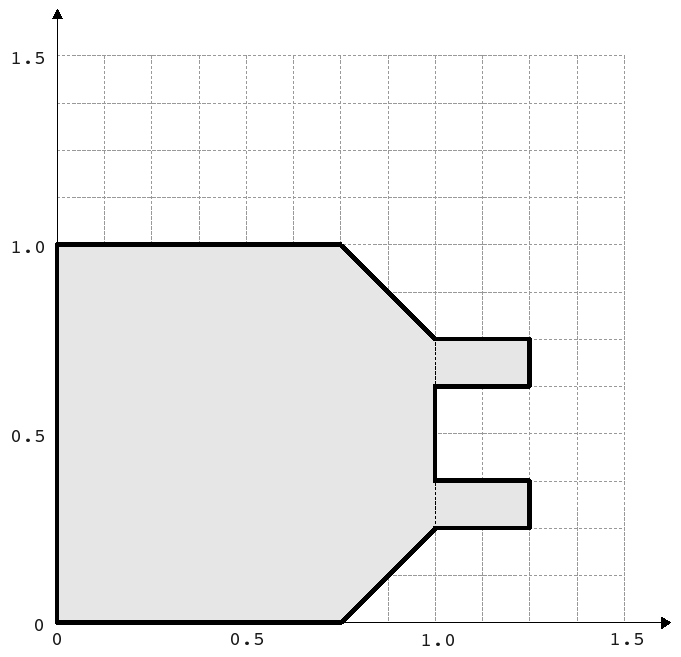
\includegraphics[width=0.6\linewidth]{./pics/robot_building/bigbob2.png} 
	\caption{The new shape of Bigbob.}
	\label{fig:bigbobteeth}
\end{figure}

To declare the size of the robot you use the \verb|size [width height]| parameter, this will cause the polygon described to be scaled to fit into a box which is \verb|width x height| in size. The default size is 1 x 1 metre, so because the addition of rubbish-collecting teeth made Bigbob longer, the size parameter was needed to stop \plst from making the robot smaller than it should be. In this way we could have specified the polygon coordinates to be 4 times the distance apart and then declared its size to be \verb|1.25 x 1| metres, and we would have got a robot the size we wanted. For a robot as large as Bigbob this is not really important, but it could be useful when building models of very small robots. 
It should be noted that it doesn't actually matter where in the cartesian coordinate system you place the polygon, instead of starting at \verb|(0, 0)| it could just as easily have started at \verb|(-1000, 12345)|. With the polygon parameter we just describe the \emph{shape} of the robot, not its size or location in the map. \newline
You may have noticed that in figures \ref{fig:basicbigbob} and \ref{fig:bigbobteeth} Bigbob is facing to the right of the grid. When you place any item in a \plst simulation they are, by default, facing to the right hand side of the simulation. Figure \ref{fig:guigrid} shows that the grids use a typical Cartesian coordinate system, and so if you want to alter the direction an object in the simulation is pointing (its ``yaw'') any angles you give use the x-axis as a reference, just like vectors in a Cartesian coordinate system (see figure \ref{fig:emptycartgrid}) and so the default yaw is $0^{\circ}$. This is also why in section \ref{sec:emptyWorld} the \verb|gui_nose| shows the map is facing to the right. Figure \ref{fig:yaws} shows a few examples of robots with different yaws.

\begin{figure}
	\centering
	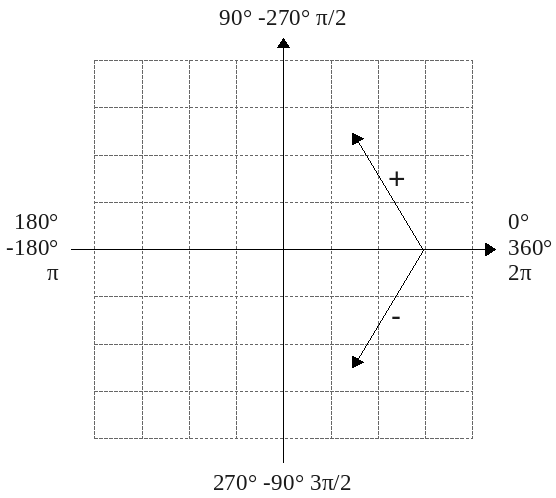
\includegraphics[width=0.5\linewidth]{./pics/robot_building/cartesian_grid_wpolars.png} 
	\caption{A cartesian grid showing how angles are described.}
	\label{fig:emptycartgrid}
\end{figure}

\begin{figure}
	\centering
	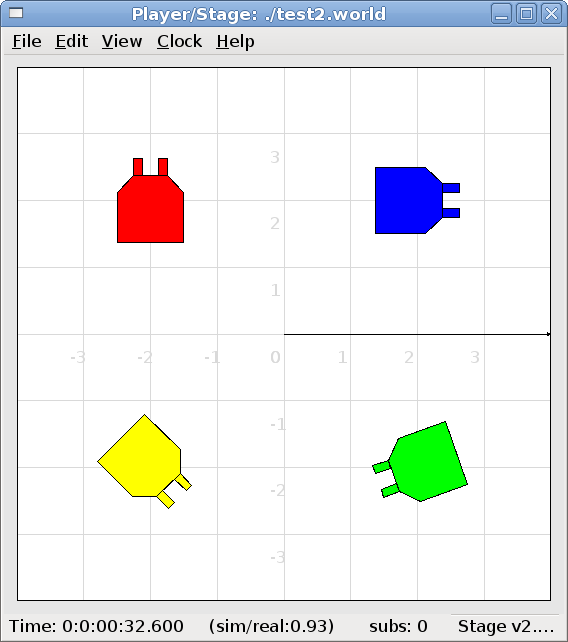
\includegraphics[width=0.6\linewidth]{./pics/robot_building/yaw_examples.png} 
	\caption{Starting from the top right robot and working anti-clockwise, the yaws of these robots are 0, 90, -45 and 200.}
	\label{fig:yaws}
\end{figure}

By default, \plst assumes the robot's centre of rotation is at its geometric centre based on what values are given to the robot's \verb|size| parameter. Bigbob's \verb|size| is \verb|1.25 x 1| so \plst will place its centre at \verb|(0.625, 0.5)|, which means that Bigbob's wheels would be closer to its teeth. Instead let's say that Bigbob's centre of rotation is in the middle of its main body (shown in figure \ref{fig:basicbigbob}) which puts the centre of rotation at \verb|(0.5, 0.5)|. To change this in robot model you use the \verb|origin [x-offset y-offset z-offset]| command:
\begin{verbatim}
define bigbob position
(
      # actual size
      size [1.25 1]
      # centre of rotation offset
      origin [0.125 0 0]

      # the shape of Bigbob
      polygons 3
      ...
      ...
      ...
)
\end{verbatim}

Finally we will specify the \verb|mass| and \verb|drive| of Bigbob, these are both parameters of the \verb|position| model and have been described earlier.
\begin{verbatim}
define bigbob position
(
      # actual size
      size [1.25 1]
      # centre of rotation offset
      origin [0.125 0 0]

      # the shape of Bigbob
      polygons 3
      ...
      ...
      ...
      
      # positonal things
      mass 10.0
      drive "diff"
)
\end{verbatim}

\paragraph{The Robot's Sensors}\label{sec:examplerobotsensors}
Now that Bigbob's body has been built let's move on to the sensors. We will put sonar and blobfinding sensors onto Bigbob so that it can detect walls and see coloured blobs it can interpret as rubbish to collect. We will also put a laser between Bigbob's teeth so that it can detect when an item passes in between them.

We will start with the sonars. The first thing to do is to define a model for the sonar array that is going to be attached to Bigbob:
\begin{verbatim}
define bigbobs_sonars ranger
(
      # parameters...
)
\end{verbatim}
Here we tell \plst that we will \verb|define| a set of sonar sensors called \verb|bigbobs_sonars| and we're using the model type \verb|ranger| to tell \plst that this is a model of some ranging devices. Let's put four sonars on Bigbob, one on the front of each tooth, and one on the front left and the front right corners of its body. 

When building Bigbob's body we were able to use any location on a coordinate grid that we wanted and could declare our shape polygons to be any distance apart we wanted so long as we resized the model with \verb|size|. In contrast, sensors - all sensors not just rangers - must be positioned according to the \emph{robot's} origin and actual size. To work out the distances in metres it helps to do a drawing of where the sensors will go on the robot and their distances from the robot's origin. When we worked out the shape of Bigbob's body we used its actual size, so we can use the same drawings again to work out the distances of the sensors from the origin as shown in figure \ref{fig:sonardrawing}.

\begin{figure}
	\centering
	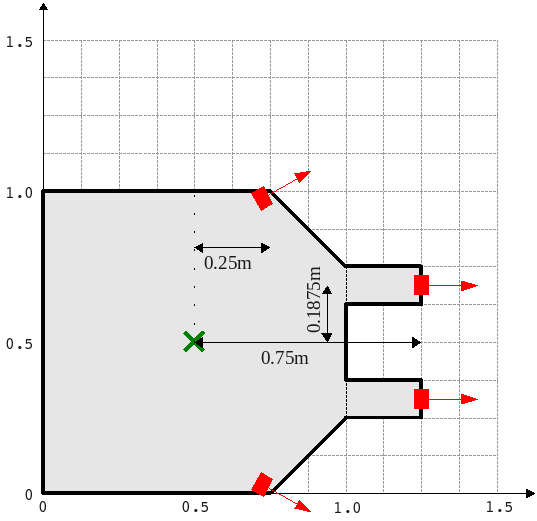
\includegraphics[width=0.6\linewidth]{./pics/robot_building/bigbob_sonars.png} 
	\caption{The position of Bigbob's sonars (in red) relative to its origin. The origin is marked with a cross, some of the distances from the origin to the sensors have been marked. The remaining distances can be done by inspection.}
	\label{fig:sonardrawing}
\end{figure}

Now we know how many sensors we want, and their coordinates relative to the origin we can begin to build our model of the sonar array. Here we will use the \verb|scount| and \verb|spose| parameters mentioned in \ref{sec:ranger}. The values for \verb|spose| are \verb|[x y yaw]|, remember that yaw is in degrees and is measured relative to the $x$ axis.
\begin{verbatim}
define bigbobs_sonars ranger
(
      # number of sonars
      scount 4

      # define the pose of each transducer [xpos ypos heading]
      spose[0] [ 0.75 0.1875 0 ]	#fr left tooth
      spose[1] [ 0.75 -0.1875 0 ]	#fr right tooth
      spose[2] [ 0.25 0.5 30]		# left corner
      spose[3] [ 0.25 -0.5 -30]		# right corner

)
\end{verbatim}

The process of working out where the sensors go relative to the origin of the robot is the most complicated part of describing the sensor, the rest is easy. To define the size, range and field of view of the sonars we just consult the sonar device's datasheet.
\begin{verbatim}
define bigbobs_sonars ranger
(
      # number of sonars
      scount 4

      # define the pose of each transducer [xpos ypos heading]
      spose[0] [ 0.75 0.1875 0 ]	#fr left tooth
      spose[1] [ 0.75 -0.1875 0 ]	#fr right tooth
      spose[2] [ 0.25 0.5 30]		# left corner
      spose[3] [ 0.25 -0.5 -30]		# right corner
      
      # define the field of view of each transducer 
      # [range_min range_max view_angle]
      sview [0.3 2.0 10]

      # define the size of each transducer [xsize ysize] in metres
      ssize [0.01 0.05]
)
\end{verbatim}

Now that Bigbob's sonars are done we will attached a blobfinder:
\begin{verbatim}
define bigbobs_eyes blobfinder
(
      # parameters
)
\end{verbatim}

Bigbob is a rubbish-collector so here we should tell it what colour of rubbish to look for. Let's say that the intended application of Bigbob is in an orange juice factory and he picks up any stray oranges or juice cartons that fall on the floor. Oranges are orange, and juice cartons are (let's say) dark blue so Bigbob's blobfinder will look for these two colours:
\begin{verbatim}
define bigbobs_eyes blobfinder
(
      # number of colours to look for
      colors_count 2
      
      # which colours to look for
      colors ["orange" "DarkBlue"]
)
\end{verbatim}
Then we define the properties of the camera, again these come from a datasheet:
\begin{verbatim}
define bigbobs_eyes blobfinder
(
      # number of colours to look for
      colors_count 2
      
      # which colours to look for
      colors ["orange" "DarkBlue"]

      # camera parameters
      image [160 120]		#resolution
      range 5.00
      fov 3.14159/3	# 60 degrees = pi/3 radians
)
\end{verbatim}
In Stage 2.X.X the following code should be used instead:
\begin{verbatim}
# bigbob's blobfinder
define bigbobs_eyes ptz
(
      blobfinder
      (
            # number of colours to look for
            channels_count 2

            # which colours to look for
            channels ["orange" "DarkBlue"]
	
            # camera parameters
            image [160 120]		#resolution
            range_max 5.00
            ptz [0 0 60]
      )
)
\end{verbatim}

The last sensor that needs adding to Bigbob is the laser, which will be used to detect whenever a piece of rubbish has been collected. Following the same principles as for our previous sensor models we can create a description of this laser:
\begin{verbatim}
define bigbobs_laser laser
(
      range_min 0.0
	
      # distance between teeth in metres
      range_max 0.25
	
      fov 3.14159/9	# 20 degrees = pi/9 radians
      # fov 20	# use this line instead of above if using stage 2.X.X
      
      pose [0.625 0.125 270]
      size [0.025 0.025]
)
\end{verbatim}
With this laser we've set its maximum range to be the distance between teeth, and the field of view is arbitrarily set to $20^{\circ}$. We have calculated the laser's \verb|pose| in exactly the same way as the sonars \verb|spose|, by measuring the distance from the laser's centre to the robot's centre of rotation, the laser's yaw is set to $270^{\circ}$ so that it points across Bigbob's teeth. We also set the size of the laser to be 2.5cm square so that it doesn't obstruct the gap between Bigbob's teeth.


\begin{figure}
	\centering
	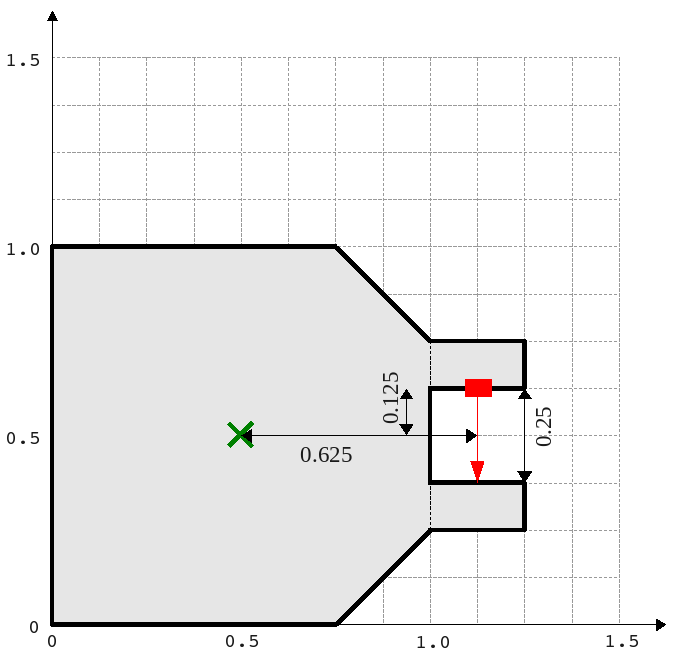
\includegraphics[width=0.6\linewidth]{./pics/robot_building/bigbob_laser.png} 
	\caption{The position of Bigbob's laser (in red) and its distance, in metres, relative to its origin (marked with a cross).}
	\label{fig:laserdrawing}
\end{figure}


Now that we have a robot body and sensor models all we need to do is put them together and place them in the world. To add the sensors to the body we need to go back to the \verb|bigbob position| model:
\begin{verbatim}
define bigbob position
(
      # actual size
      size [1.25 1]
      # centre of rotation offset
      origin [0.125 0 0]

      # the shape of Bigbob
      polygons 3
      ...
      ...
      ...
      
      # positonal things
      mass 10.0
      drive "diff"
      
      # sensors attached to bigbob
      bigbobs_sonars()
      bigbobs_eyes()
      bigbobs_laser()
)
\end{verbatim}
The extra line \verb|bigbobs_sonars()| adds the sonar model called \verb|bigbobs_sonars()| onto the \verb|bigbob| model, likewise for \verb|bigbobs_eyes()| and \verb|bigbobs_laser()|. After this final step we now have a complete model of our robot bigbob, the full code for which can be found in appendix A. At this point it's worthwhile to copy this into a .inc file, so that the model could be used again in other simulations or worlds.\newline
To put our Bigbob model into our empty world (see section \ref{sec:basicWorldfile}) we need to add the robot to our worldfile empty.world:
\begin{verbatim}
include "map.inc"
include "bigbob.inc"

# size of the whole simulation
size [15 15]


# configure the GUI window
window
( 
      size [ 700.000 700.000 ] 
      scale 0.025
)


# load an environment bitmap
map
(
      bitmap "bitmaps/cave.png"
      size [15 15]	
)

bigbob
(
      name "bob1"
      pose [-5 -6 45]
      color "red"
)
\end{verbatim}
Here we've put all the stuff that describes Bigbob into a .inc file \verb|bigbob.inc|, and when we include this, all the code from the .inc file is inserted into the .world file. The section here is where we put a version of the bigbob model into our world:
\begin{verbatim}
bigbob
(
      name "bob1"
      pose [-5 -6 45]
      color "green"
)
\end{verbatim}
Bigbob is a model description, by not including any \verb|define| stuff in the top line there it means that we are making an instantiation of that model, with the name \verb|bob1|. Using an object-oriented programming analogy, \verb|bigbob| is our class, and \verb|bob1| is our object of class \verb|bigbob|. The \verb|pose [x y yaw]| parameter works in the same was as \verb|spose [x y yaw]| does. The only differences are that the coordinates use the centre of the simulation as a reference point and \verb|pose| lets us specify the initial position and heading of the entire \verb\bob1\ model, not just one sensor within that model.
Finally we specify what colour \verb|bob1| should be, by default this is red. The \verb|pose| and \verb|color| parameters could have been specified in our bigbob model but by leaving them out it allows us to vary the colour and position of the robots for each different robot of type \verb|bigbob|, so we could declare multiple robots which are the same size, shape and have the same sensors, but are rendered by \plst in different colours and are initialised at different points in the map.\newline
When we run the new empty.world with \plst we see our Bigbob robot is occupying the world, as shown in figure \ref{fig:finalRobotBuild}. The dark mark on top of the robot is the blobfinder camera.

\begin{figure}
	\centering
	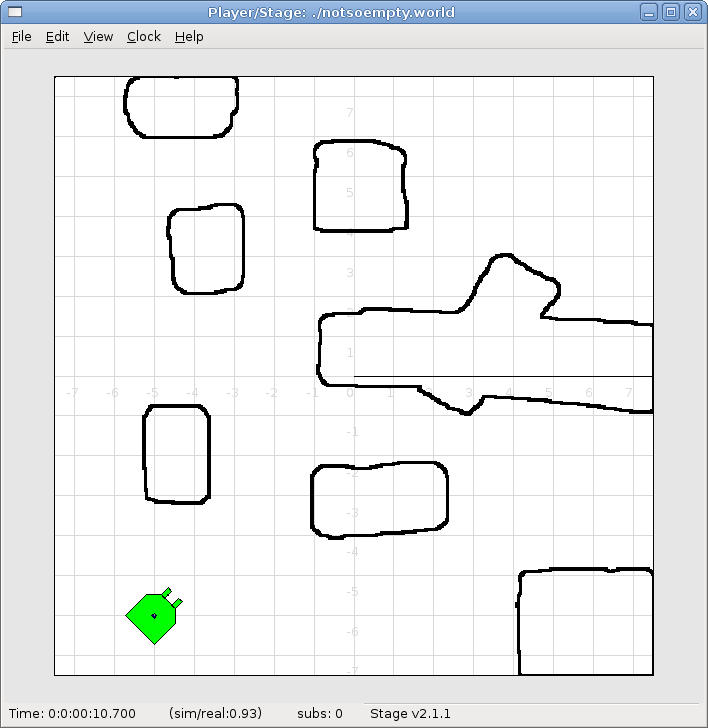
\includegraphics[width=0.7\linewidth]{./pics/robot_building/final_robot_build.png} 
	\caption{Our bob1 robot placed in the empty world.}
	\label{fig:finalRobotBuild}
\end{figure}


\subsection{Building Other Stuff} \label{sec:otherStuff}
We established in section \ref{sec:examplerobotsensors} that Bigbob works in a orange juice factory collecting oranges and juice cartons. Now we need to build models to represent the oranges and juice cartons so that Bigbob can interact with things.

We'll start by building a model of an orange:
\begin{verbatim}
define orange model
(
      # parameters...
)
\end{verbatim}
The first thing to define is the shape of the orange. The \verb|polygons| parameter is one way of doing this, which we can use to build a blocky approximation of a circle. An alternative to this is to use \verb|bitmap| which we previously saw being used to create a map. What the bitmap command actually does is take in a picture, and turn it into a series of polygons which are connected together to make a model the same shape as the picture. This is illustrated in figure \ref{fig:ghosts}. To get rid of the blocks' outlines add \verb|gui_outline 0| to the model description, with the large ghost in figure \ref{fig:ghosts} it's not so much of a problem, but with smaller models, like an orange, the black outlines prevent the model's colour from being visible.

\begin{figure}
	\centering
	\begin{minipage}[c]{0.3\linewidth}
		\centering
		
\includegraphics{./pics/oranges_box/ghost_original.png} %[width=\linewidth]
		
	\end{minipage}%
	\hspace{0.05\linewidth}
	\begin{minipage}[c]{0.6\linewidth}
		\centering
		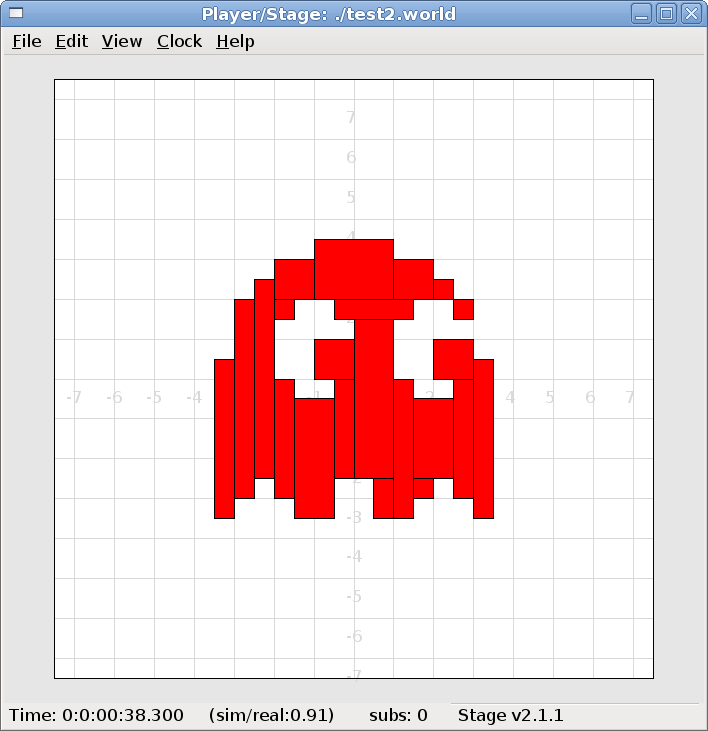
\includegraphics[width=\linewidth]{./pics/oranges_box/ghost_woutline.png} 
	\end{minipage}	
	\caption{The left image is the original picture, the right image is its \plst interpretation.}
		\label{fig:ghosts}
\end{figure}

\begin{verbatim}
define orange model
(
      bitmap "bitmaps/circle.png"
      size [0.15 0.15]
      color "orange"
      
      gui_outline 0
      gripper_return 1
)
\end{verbatim}
In this code we describe a model called \verb|orange| which uses a bitmap to define its shape and represents an object which is 15cm by 15cm and coloured orange. The \verb|gripper_return| parameter is a special type of \_return because it means that the model can be grabbed by a robot's gripper but it \emph{also} means the object can be pushed a little bit in the simulation. We want our orange model to be pushable so, even though Bigbob has no gripper, the orange's \verb|gripper_return| parameter is set to true. Figure \ref{fig:orangeandbob} shows our orange model next to Bigbob.
\begin{figure}
	\centering
	\begin{minipage}[c]{0.2\linewidth}
		\centering
		
\includegraphics{./pics/oranges_box/circle.png} 
		\caption{./bitmaps/circle.png}
		\label{fig:circle.png}	
	\end{minipage}%
	\hspace{0.1\linewidth}
	\begin{minipage}[c]{0.6\linewidth}
		\centering
		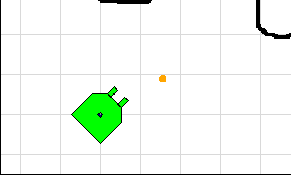
\includegraphics[width=\linewidth]{./pics/oranges_box/orange_and_bob.png} 
		\caption{The orange model rendered in the same \plst window as Bigbob.}
		\label{fig:orangeandbob}
	\end{minipage}	
\end{figure}

Building a juice carton model is similarly quite easy:
\begin{verbatim}
define carton model
(
      # a carton is retangular
      # so make a square shape and use size[]
      polygons 1
      polygon[0].points 4
      polygon[0].point[0] [0 0]
      polygon[0].point[1] [0 1]
      polygon[0].point[2] [1 1]
      polygon[0].point[3] [1 0]
	
      # average carton size is ~ 20cm x 10cm x 5cm
      size [0.1 0.2]
	
      color "DarkBlue"
      gripper_return 1
)
\end{verbatim}

We can use the \verb|polygons| command since juice cartons are boxy, with boxy things it's slightly easier to describe the shape with \verb|polygon| than drawing a bitmap and using that.\newline

Now that we have described basic \verb|orange| and \verb|carton| models it's time to put some oranges and cartons into the simulation. This is done in the same way as our example robot was put into the world:
\begin{verbatim}
orange
(
      name "orange1" 
      pose [-2 -5 0]
)

carton
(
      name "carton1" 
      pose [-3 -5 0]
)
\end{verbatim}
We created models of oranges and cartons, and now we are declaring that there will be an instance of these models (called \verb|orange1| and \verb|carton1| respectively) at the given positions. Unlike with the robot, we declared the \verb|color| of the models in the description so we don't need to do that here. If we did have different colours for each orange or carton then it would mess up the blobfinding on Bigbob because the robot is only searching for orange and dark blue.
At this point it would be useful if we could have more than just one orange or carton in the world (Bigbob would not be very busy if there wasn't much to pick up), it turns out that this is also pretty easy:
\begin{verbatim}
orange(name "orange1" pose [-1 -5 0])
orange(name "orange2" pose [-2 -5 0])
orange(name "orange3" pose [-3 -5 0])
orange(name "orange4" pose [-4 -5 0])

carton(name "carton1" pose [-2 -4 0])
carton(name "carton2" pose [-2 -3 0])
carton(name "carton3" pose [-2 -2 0])
carton(name "carton4" pose [-2 -1 0])
\end{verbatim}

Up until now we have been describing models with each parameter on a new line, this is just a way of making it more readable for the programmer -- especially if there are a lot of parameters. If there are only a few parameters or you want to repeat the code (as we've done here) it can all be put onto one line. Here we declare that there will be four \verb|orange| models in the simulation with the names \verb|orange1| to \verb|orange4|, we also need to specify different poses for the models so they aren't all on top of each other. Properties that the orange models have in common (such as shape, colour or size) should all be in the model definition. 

The full worldfile is included in appendix B, this includes the orange and carton models as well as the code for putting them in the simulation. Figure \ref{fig:finalRobotandStuff} shows the populated \plst simulation.

\begin{figure}
	\centering
	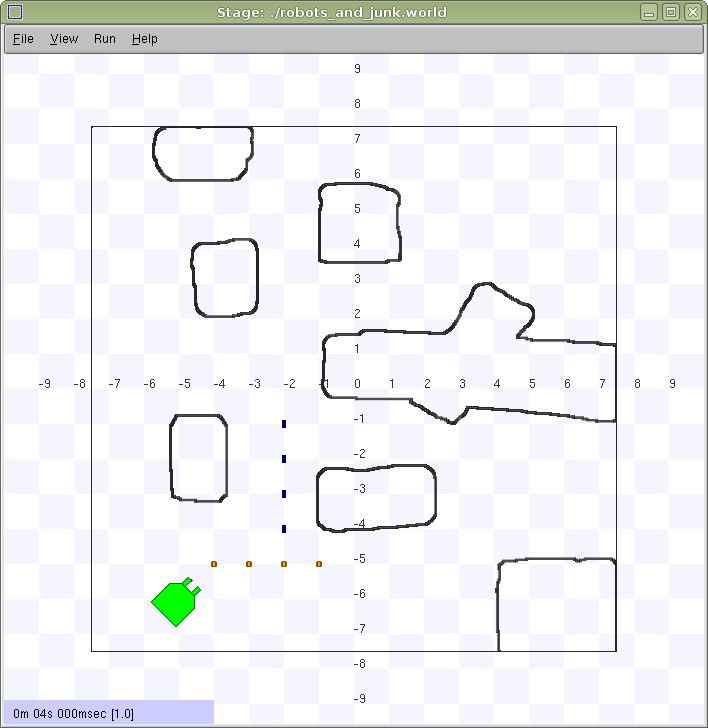
\includegraphics[width=0.7\linewidth]{./pics/oranges_box/final_robot_and_stuff.png} 
	\caption{The Bigbob robot placed in the simulation along with junk for it to pick up.}
	\label{fig:finalRobotandStuff}
\end{figure}

\section{Writing a Configuration (.cfg) File} \label{sec:WritingConfigurationFile}

As mentioned earlier, \pl is a hardware abstraction layer which connects your code to the robot's hardware. It does this by acting as a Server/Client type program where your code and the robot's sensors are clients to a \pl server which then passes the data and instructions around to where it all needs to go. This stuff will be properly explained in section \ref{sec:coding}, it all sounds more complicated than it is because \plst takes care of all the difficult stuff. The configuration file is needed in order to tell the \pl server which drivers to use and which interfaces the drivers will be using.

For each model in the simulation or device on the robot that you want to interact with, you will need to specify a driver. This is far easier than writing worldfile information, and follows the same general syntax. The driver specification is in the form:
\begin{verbatim}
driver
(
      name "driver_name"
      provides [device_address]
      # other parameters... 
)
\end{verbatim}
The \verb|name| and \verb|provides| parameters are mandatory information, without them \pl won't know which driver to use (given by \verb|name|) and what kind of information is coming from the driver (\verb|provides|). The \verb|name| parameter is not arbitrary, it must be the name of one of \pl's inbuilt drivers\footnote{It is also possible to build your own drivers for a hardware device but this document won't go into how to do this because it's not relevant to \plst.} that have been written for \pl to interact with a robot device. A list of supported driver names is in the \pl Manual\footnote{http://playerstage.sourceforge.net/doc/\pl-2.1.0/player/group\_\_drivers.html}, although when using Stage the only one that is needed is \verb|"stage"|. 

The \verb|provides| parameter is a little more complicated than \verb|name|. It is here that you tell \pl what interface to use in order to interpret information given out by the driver (often this is sensor information from a robot), any information that a driver \verb\provides\ can be used by your code. For a Stage simulated robot the \verb|"stage"| driver can provide the interfaces to the sensors discussed in section \ref{sec:robotSensors}. Each interface shares the same name as the sensor model, so for example a \verb|ranger| model would use the \verb|ranger| interface to interact with \pl and so on (the only exception to this being the \verb|position| model which uses the \verb|position2d| interface). The \pl manual contains a list of all the different interfaces that can be used\footnote{http://playerstage.sourceforge.net/doc/\pl-2.1.0/player/group\_\_interfaces.html}, the most useful ones have already been mentioned in section \ref{sec:robotSensors}, although there are others too numerable to list here.

The input to the \verb|provides| parameter is a ``device address'', which specifies which TCP port an interface to a robot device can be found, section \ref{sec:deviceAddress} has more information about device addresses. This uses the key:host:robot:interface:index form separated by white space.

\begin{verbatim}
provides ["key:host:robot:interface:index" 
          "key:host:robot:interface:index"
          "key:host:robot:interface:index"
          ...]
\end{verbatim}

After the two mandatory parameters, the next most useful driver parameter is \verb|model|. This is only used if \verb|"stage"| is the driver, it tells \pl which particular model in the worldfile is providing the interfaces for this particular driver. A different driver is needed for each model that you want to use. Models that aren't required to do anything (such as a map, or in the example of section \ref{sec:otherStuff} oranges and boxes) don't need to have a driver written for them.\newline
The remaining driver parameters are \verb|requires| and \verb|plugin|. The \verb|requires| is used for drivers that need input information such as \verb|"vfh"|, it tells this driver where to find this information and which interface it uses. The \verb|requires| parameter uses the same key:host:robot:interface:index syntax as the \verb|provides| parameter. Finally the \verb|plugin| parameter is used to tell \pl where to find all the information about the driver being used. Earlier we made a .cfg file in order to create a simulation of an empty (or at least unmoving) world, the .cfg file read as follows:
\begin{verbatim}
driver
(		
      name "stage"
      plugin "libstageplugin"

      provides ["simulation:0" ]

      # load the named file into the simulator
      worldfile "empty.world"	
)
\end{verbatim}
This has to be done at the beginning of the configuration file because it tells \pl that there is a driver called \verb|"stage"| that we're going to use and the code for dealing with this driver can be found in the \verb|libstageplugin| plugin. This needs to be specified for Stage because Stage is an add-on for \pl, for drivers that are built into \pl by default the \verb|plugin| doesn't need to be specified.

\subsection{Device Addresses - key:host:robot:interface:index} \label{sec:deviceAddress}

A device address is used to tell \pl where the driver you are making will present (or receive) information and which interface to use in order to read this information. This is a string in the form \verb|key:host:robot:interface:index| where each field is separated by a colon.
\begin{itemize}
\item \verb\key\: The \pl manual states that: \textit{``The purpose of the key field is to allow a driver that supports multiple interfaces of the same type to map those interfaces onto different devices''}\cite{PlayerManualDeviceAddresses}. This is a driver level thing and has a lot to do with the \verb\name\ of the driver that you are using, generally for \verb\"stage"\ the \verb\key\ doesn't need to be used. If you're using \pl without Stage then there is a useful section about device address keys in the \pl manual\footnote{http://playerstage.sourceforge.net/doc/\pl-2.1.0/player/group\_\_tutorial\_\_config.html\#device\_key}.
\item \verb\host\: This is the address of the host computer where the device is located. With a robot it could be the IP address of the robot. The default host is ``localhost'' which means the computer on which \pl is running.
\item \verb\robot\: this is the TCP port through which \pl should expect to receive data from the interface usually a single robot and all its necessary interfaces are assigned to one port. The default port used is 6665, if there were two robots in the simulation the ports could be 6665 and 6666 although there's no rule saying which number ports you can or can't use.
\item \verb\interface\: The interface to use in order to interact with the data. There is no default value for this option because it is a mandatory field.
\item \verb\index\: If a robot has multiple devices of the same type, for instance it has 2 cameras to give the robot depth perception, each device uses the same interface but gives slightly different information. The index field allows you to give a slightly different address to each device. So two cameras could be \verb|camera:0| and \verb|camera:1|. This is very different from the \verb\key\ field because having a ``driver that supports multiple interfaces of the same type'' is NOT the same as having multiple devices that use the same interface. Again there is no default index, as this is a mandatory field in the device address, but you should use 0 as the index if there is only one of that kind of device. 
\end{itemize}
If you want to use any of the default values it can just be left out of the device address. So we could use the default host and robot port and specify (for example) a laser interface just by doing \verb\"laser:0"\. However, if you want to specify fields at the beginning of the device address but not in the middle then  the separating colons should remain. For example if we had a host at \verb|"127.0.0.1"| with a \verb\laser\ interface then we would specify the address as \verb|"127.0.0.1::laser:0"|, the robot field is empty but the colons around it are still there. You may notice that the key field here was left off as before.

\subsection{Putting the Configuration File Together}\label{sec:finishConfigs}

We have examined the commands necessary to build a driver for a model in the worldfile, now it is just a case of putting them all together. To demonstrate this process we will build a configuration file for the worldfile developed in section \ref{sec:BuildingAWorld}. In this world we want our code to be able to interact with the robot, so in our configuration file we need to specify a driver for this robot.
\begin{verbatim}
driver
(
      # parameters... 
)
\end{verbatim}

The inbuilt driver that \plst uses for simulations is called \verb|"stage"| so the driver name is \verb|"stage"|.
\begin{verbatim}
driver
(
      name "stage"
)
\end{verbatim}
The Bigbob robot uses \verb|position|, \verb|laser|, \verb|blobfinder| and \verb|ranger| sensors. These correspond to the \verb|position2d|, \verb|laser|, \verb|blobfinder| and  interfaces respectively. The \verb|ranger| sensor is a special case because the ranger interface has not currently been implemented (for versions Stage 3.0.1 or earlier). To work around this you'll need to use the \verb\sonar\ interfaces instead (there is apparently an IR interface which could be used instead of \verb\ranger\, but it doesn't seem to work on either Stage 2 or Stage 3). 

We want our code to be able to read from these sensors, so we need to declare interfaces for them and tell \pl where to find each device's data, for this we use the configuration file's \verb\provides\ parameter. This requires that we construct device addresses for each sensor; to remind ourselves, this is in the key:host:robot:interface:index format. We aren't using any fancy drivers, so we don't need to specify a key. We are running our robot in a simulation on the same computer as our \pl sever, so the host name is \verb\localhost\ which is the default, so we also don't need to specify a host. The robot is a TCP port to receive robot information over, picking which port to use is pretty arbitrary but what usually happens is that the first robot uses the default port 6665 and subsequent robots use 6666, 6667, 6668 etc. There is only one robot in our simulation so we will use port 6665 for all our sensor information from this robot. 
We only have one sensor of each type, so our devices don't need separate indices. What would happen if we did have several sensors of the same type (like say two cameras) is that we put the first device at index 0 and subsequent devices using the same interface have index 1, then 2, then 3 and so on.\footnote{There are lots of ranger sensors in our model but when we created the robot's sensors in section \ref{sec:examplerobotsensors} we put them all into the same ranger model. So as far as the configuration file is concerned there is only one raging device using either the sonar or IR interface, because all the separate ranger devices are lumped together into this one model. We don't need to declare each ranger on an index of its own.}  
Finally we use interfaces appropriate to the sensors the robot has, so in our example these are the \verb|position|, \verb|laser|, \verb|blobfinder| interfaces and for our \verb\ranger\ devices we will use \verb\sonar\.

Putting all this together under the \verb\provides\ parameter gives us:
\begin{verbatim}
driver
(
  name "stage"
  provides ["6665:position2d:0" 
            "6665:sonar:0" 
            "6665:blobfinder:0" 
            "6665:laser:0" ]
)
\end{verbatim}
The device addresses can be on the same line as each other or separate lines, just so long as they're separated by some form of white space.

The last thing to do on our driver is the \verb|model "model_name"| parameter which needs to be specified because we are using \plst. This tells the simulation software that anything you do with this driver will affect the model \verb\"model_name"\ in the simulation. In the simulation we built we named our robot model ``bob1'', so our final driver for the robot will be:
\begin{verbatim}
driver
(
      name "stage"
      provides ["6665:position2d:0" 
            "6665:sonar:0" 
            "6665:blobfinder:0" 
            "6665:laser:0"]
      model "bob1" 
)
\end{verbatim}
If our simulation had multiple Bigbob robots in, the configuration file drivers would be very similar to one another. If we created a second robot in our worldfile and called it ``bob2'' then the driver would be:
\begin{verbatim}
driver
( 
      name "stage" 
      provides ["6666:position2d:0" 
            "6666:sonar:0" 
            "6666:blobfinder:0" 
            "6666:laser:0"]
      model "bob2" 
)
\end{verbatim}
Notice that the port number and model name are the only differences because the robots have all the same sensors.

A driver of this kind can be built for any model that is in the worldfile, not just the robots. For instance a map driver can be made which uses the \verb\map\ interface and will allow you to get size, origin and occupancy data about the map. The only requirement is that if you want to do something to the model with your code then you need to build a driver for it in the configuration file. Finally when we put the bit which declares the \verb\stage\ driver (this part is compulsory for any simulation configuration file) together with our drivers for the robot we end up with our final configuration file:
\begin{verbatim}
driver
(		
      name "stage"
      plugin "libstageplugin"

      provides ["simulation:0" ]

      # load the named file into the simulator
      worldfile "worldfile_name.world"	
)      

driver
(
      name "stage"
      provides ["6665:position2d:0" 
            "6665:sonar:0" 
            "6665:blobfinder:0" 
            "6665:laser:0"]
      model "bob1" 
)
\end{verbatim}

\section{Getting Your Simulation To Run Your Code}\label{sec:coding}

To learn how to write code for \pl or \plst it helps to understand the basic structure of how \pl works. \pl uses a Server/Client structure in order to pass data and instructions between your code and the robot's hardware. \pl is a server, and a hardware device\footnote{remember, a device is a piece of hardware that uses a driver which conforms to an interface. See section \ref{sec:interfaceDriverDevices}} on the robot is subscribed as a client to the server via a thing called a \emph{proxy}. The .cfg file associated with your robot (or your simulation) takes care of telling the \pl server which devices are attached to it, so when we run the command \verb\player some_cfg.cfg\ this starts up the \pl server and connects all the necessary hardware devices to the server. Figure \ref{fig:serverclientRobot} shows a basic block diagram of the structure of \pl when implemented on a robot. In \plst the same command will start the \pl server and load up the worldfile in a simulation window, this runs on your computer and allows your code to interact with the simulation rather than hardware. Figure \ref{fig:serverclientSim} shows a basic block diagram of the \plst structure.
Your code must also subscribe to the \pl server so that it can access these proxies and hence control the robot. \pl has functions and classes which will do all this for you, but you still need to actually call these functions with your code and know how to use them. 

\begin{figure}
 	\centering
	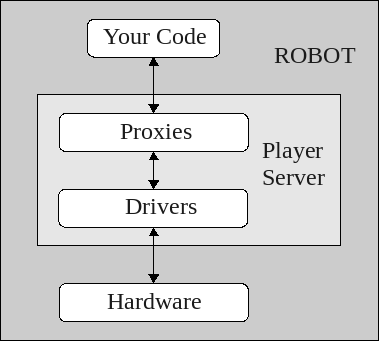
\includegraphics[width=0.6\linewidth]{pics/coding/ServerClient_robot.png}
	\caption{The server/client control structure of \pl when used on a robot. There may be several proxies connected to the server at any time.}
	\label{fig:serverclientRobot}
\end{figure} 

\begin{figure}
 	\centering
	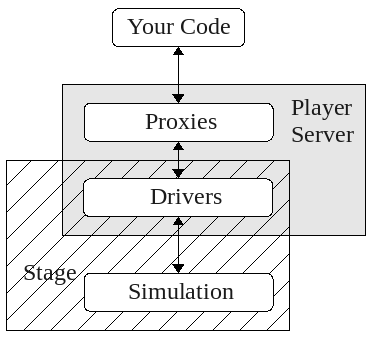
\includegraphics[width=0.6\linewidth]{pics/coding/ServerClient_sim.png}
	\caption{The server/client control structure of \plst when used as a simulator. There may be several proxies connected to the server at any time.}
	\label{fig:serverclientSim}
\end{figure} 

\pl is compatable with C, C++ or Python code, however in this manual we will only really be using C++ because it is the simplest to understand. The process of writing \pl code is mostly the same for each different language though. The \pl and \pl proxy functions have different names for each language, but work in more or less the same way, so even if you don't plan on using C++ or Stage this section will still contain helpful information.

Before beginning a project it is highly recommended that for any programs other than basic examples you should always wrap your \pl commands around your own functions and classes so that all your code's interactions with \pl are kept together the same file. This isn't a requirement of \pl, it's just good practice. For example, if you upgrade \pl or if for some reason your robot breaks and a certain function no longer works you only have to change part of a file instead of searching through all your code for places where \pl functions have been used.

Finally, in order to compile your program you use the following commands (in Linux):\newline
\texttt{g++ -o example0 \`{}pkg-config --cflags playerc++\`{} example0.cc \`{}pkg-config --libs playerc++\`{}}

That will compile a program to a file called \verb\example0\ from the C++ code file \verb\example0.cc\. If you are coding in C instead then use the following command:\newline
\texttt{gcc -o example0 \`{}pkg-config --cflags playerc\`{} example0.c \`{}pkg-config --libs playerc\`{} }

\subsection{Connecting to the Server and Proxies With Your Code}\label{sec:connectingtoserver}

The first thing to do within your code is to include the \pl header file. Assuming \plst is installed correctly on your machine then this can be done with the line \verb\#include <libplayerc++/playerc++.h>\ (if you're using C then type \verb\#include <libplayerc/playerc.h>\ instead).

Next we need to establish a \pl Client, which will interact with the \pl server for you. To do this we use the line:
\begin{verbatim}
PlayerClient client_name(hostname, port); 
\end{verbatim}
What this line does is declare a new object which is a PlayerClient called \verb\client_name\ which connects to the \pl server at the given address. The hostname and port is like that discussed in section \ref{sec:deviceAddress}. If your code is running on the same computer (or robot) as the \pl server you wish to connect to then the hostname is ``localhost'' otherwise it will be the IP address of the computer or robot. The port is an optional parameter usually only needed for simulations, it will be the same as the port you gave in the .cfg file. This is only useful if your simulation has more than one robot in and you need your code to connect to both robots. So if you gave your first robot port 6665 and the second one 6666 (like in the example of section \ref{sec:finishConfigs}) then you would need two PlayerClients, one connected to each robot, and you would do this with the following code:
\begin{verbatim}
PlayerClient robot1("localhost", 6665); 
PlayerClient robot2("localhost", 6666); 
\end{verbatim}
If you are only using one robot and in your .cfg file you said that it would operate on port 6665 then the port parameter to the PlayerClient class is not needed. 
\newline
Once we have established a PlayerClient we should connect our code to the device proxies so that we can exchange information with them. Which proxies you can connect your code to is dependent on what you have put in your configuration file. For instance if your configuration file says your robot is connected to a laser but not a camera you can connect to the laser device but not the camera, even if the robot (or robot simulation) has a camera on it. 

Proxies take the name of the interface which the drivers use to talk to \pl. Let's take part of the Bigbob example configuration file from section \ref{sec:finishConfigs}:
\begin{verbatim}
driver
(
  name "stage"
  provides ["6665:position2d:0" 
            "6665:sonar:0" 
            "6665:blobfinder:0" 
            "6665:laser:0" ]
)
\end{verbatim}
Here we've told the \pl server that our ``robot'' has devices which use the position2d, sonar, blobfinder and laser interfaces. In our code then, we should connect to the position2d, sonar, blobfinder and laser proxies like so:
\begin{verbatim}
Position2dProxy positionProxy_name(&client_name,index);
SonarProxy      sonarProxy_name(&client_name,index);
BlobfinderProxy blobProxy_name(&client_name,index);
LaserProxy      laserProxy_name(&client_name,index);
\end{verbatim}
A full list of which proxies \pl supports can be found in the \pl manual\footnote{http://playerstage.sourceforge.net/doc/Player-2.1.0/player/classPlayerCc\_1\_1ClientProxy.html}, they all follow the convention of being named after the interface they use. In the above case \verb\xProxy_name\ is the name you want to give to the proxy object, \verb\client_name\ is the name you gave the PlayerClient object earlier and \verb\index\ is the index that the device was given in your configuration file (probably 0).

\subsubsection{Setting Up Connections: an Example.}\label{sec:exampleconnectingtoserver}

For an example of how to connect to the \pl sever and device proxies we will use the example configuration file developed in section \ref{sec:finishConfigs}. For convenience this is reproduced below:
\begin{verbatim}
driver
(		
      name "stage"
      plugin "libstageplugin"

      provides ["simulation:0" ]

      # load the named file into the simulator
      worldfile "worldfile_name.world"	
)      

driver
(
      name "stage"
      provides ["6665:position2d:0" 
            "6665:sonar:0" 
            "6665:blobfinder:0" 
            "6665:laser:0"]
      model "bob1" 
)
\end{verbatim}
To set up a PlayerClient and then connect to proxies on that server we can use principles discussed in this section to develop the following code:
\begin{verbatim}
#include <stdio.h>
#include <libplayerc++/playerc++.h>

int main(int argc, char *argv[])
{
      /*need to do this line in c++ only*/
      using namespace PlayerCc;
	
      PlayerClient    robot("localhost");

      Position2dProxy p2dProxy(&robot,0);
      SonarProxy      sonarProxy(&robot,0);
      BlobfinderProxy blobProxy(&robot,0);
      LaserProxy      laserProxy(&robot,0);

      //some control code
      return 0;
}
\end{verbatim}

\subsection{Interacting with Proxies}\label{sec:interactingwithproxies}

As you may expect, each proxy is specialised towards controlling the device it connects to. This means that each proxy will have different commands depending on what it controls. 
In Player version 2.1.0 there are 38 different proxies which you can choose to use, many of which are not applicable to \plst. This manual will not attempt to explain them all, a full list of avaliable proxies and their functions is in the \pl manual\footnote{http://playerstage.sourceforge.net/doc/Player-2.1.0/player/classPlayerCc\_1\_1ClientProxy.html}, although the returns, parameters and purpose of the proxy function is not always explained. 
\newline The following few proxies are probably the most useful to anyone using \pl or \plst.

\subsubsection{Position2dProxy}
The Position2dProxy is the number one most useful proxy there is. It controls the robot's motors and keeps track of the robot's odometry (where the robot thinks it is based on how far its wheels have moved).

\paragraph{Get/SetSpeed}
The \verb\SetSpeed\ command is used to tell the robot's motors how fast to turn. There are two different \verb\SetSpeed\ commands that can be called, one is for robots that can move in any direction and the other is for robots with differential or car-like drives. 
\begin{itemize}
\item \verb\SetSpeed(double XSpeed, double YSpeed, double YawSpeed)\
\item \verb\SetSpeed(double XSpeed, double YawSpeed)\
\item \verb\SetCarlike(double XSpeed, double DriveAngle)\
\end{itemize}
\begin{figure}
	\centering
	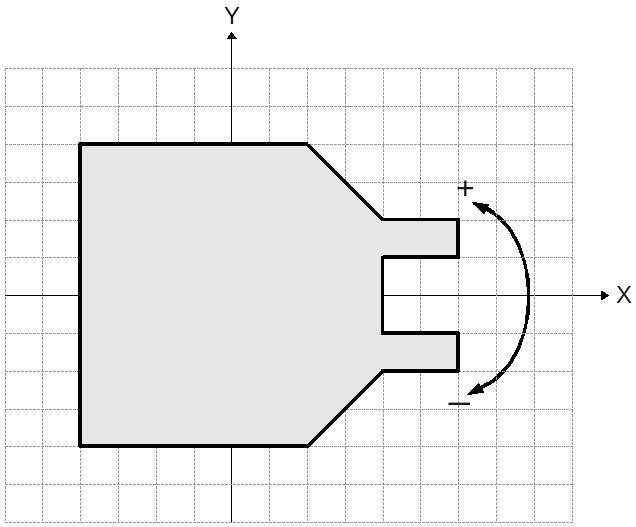
\includegraphics[width=0.6\linewidth]{./pics/coding/bob_cartgrid.png}
	\caption{A robot on a cartesian grid. This shows what directions the X and Y speeds will cause the robot to move in. A positive yaw speed will turn the robot in the direction of the + arrow, a negative yaw speed is the direction of the - arrow.}
	\label{fig:bobcartesiangrid}
\end{figure} 
Figure \ref{fig:bobcartesiangrid} shows which direction the x, y and yaw speeds are in relation to the robot. The x speed is the rate at which the robot moves forward and the y speed is the robot's speed sideways, both are to be given in metres per second. The y speed will only be useful if the robot you want to simulate or control is a ball, since robots with wheels cannot move sideways. The yaw speed controls how fast the robot is turning and is given in radians per second, \pl has an inbuilt global function called \verb\dtor()\ which converts a number in degrees into a number in radians which could be useful when setting the yaw speed. If you want to simulate or control a robot with a differential drive system then you'll need to convert left and right wheel speeds into a forward speed and a turning speed before sending it to the proxy. For car-like drives there is the \verb\SetCarlike\ which, again is the forward speed in m/s and the drive angle in radians.

The \verb\GetSpeed\ commands are essentially the reverse of the SetSpeed command. Instead of setting a speed they return the current speed relative to the robot (so x is the forward speed, yaw is the turning speed and so on).
\begin{itemize}
	\item \verb\GetXSpeed\: forward speed (metres/sec).
	\item \verb\GetYSpeed\: sideways (perpendicular) speed (metres/sec).
	\item \verb\GetYawSpeed\: turning speed (radians/sec).
\end{itemize}

\paragraph{Get\_Pos}
This function interacts with the robot's odometry. It allows you to monitor where the robot thinks it is. Coordinate values are given relative to its starting point, and yaws are relative to its starting yaw. 
\begin{itemize}
	\item \verb\GetXPos()\: gives current x coordinate relative to its x starting position.
	\item \verb\GetYPos()\: gives current y coordinate relative to its y starting position.
	\item \verb\GetYaw()\: gives current yaw relative to its starting yaw.
\end{itemize}

In section \ref{sec:position}, we specified whether it would record odometry by measuring how much its wheels have turned, or whether the robot would have perfect knowledge of its current coordinates (by default the robot does not record odometry at all). If you set the robot to record odometry using its wheels then the positions returned by these get commands will become increasingly inaccurate as the simulation goes on. If you want to log your robots position as it moves around, these functions along with the perfect odometry\footnote{See section \ref{sec:robotSensors} for how to give the robot perfect odometry.} setting can be used. 

\paragraph{SetMotorEnable()}
This function takes a boolean input, telling \pl whether to enable the motors or not. If the motors are disabled then the robot will not move no matter what commands are given to it, if the motors are enabled then the motors will always work, this is not so desirable if the robot is on a desk or something and is likely to get damaged. Hence the motors being enabled is optional. If you are using \plst, then the motors will always be enabled and this command doesn't need to be run. However, if your code is ever likely to be moved onto a real robot and the motors are not explicitly enabled in your code, then you may end up spending a long time trying to work out why your robot is not working.

\subsubsection{SonarProxy}
The sonar proxy can be used to receive the distance from the sonar to an obstacle in metres. To do this you use the command:
\begin{itemize}
 \item \verb\sonarProxy_name[sonar_number]\
\end{itemize}
Where \verb\sonarProxy_name\ is the SonarProxy object and \verb\sonar_number\ is the number of the ranger. In \plst the sonar numbers come from the order in which you described the ranger devices in the worldfile. In section \ref{sec:examplerobotsensors} we described the ranger sensors for the Bigbob robot like so:
\begin{verbatim}
define bigbobs_sonars ranger
(
      # number of sonars
      scount 4

      # define the pose of each transducer [xpos ypos heading]
      spose[0] [ 0.75 0.1875 0 ]	#fr left tooth
      spose[1] [ 0.75 -0.1875 0 ]	#fr right tooth
      spose[2] [ 0.25 0.5 30]		# left corner
      spose[3] [ 0.25 -0.5 -30]		# right corner

)
\end{verbatim}
In this example \verb\sonarProxy_name[0]\ gives us the distance from the left tooth ranger to an obstacle, \verb\sonarProxy_name[1]\ gives the distance from the front right tooth to an obstacle, and so on. If no obstacle is detected then the function will return whatever the ranger's maximum range is.

\subsubsection{LaserProxy}
A laser is a special case of ranger device, it makes regularly spaced range measurements turning from a minimum angle to a maximum angle. Each measurement, or scan point, is treated as being done with a separate ranger. Where angles are given they are given with reference to the laser's centre front (see figure \ref{fig:laserangles}).

\begin{itemize}
	\item \verb\GetCount\: The number of laser scan points that the laser measures.
	\item \verb\laserProxy_name[laser_number]\ The range returned by the \verb\laser_number\$^{th}$ scan point. Scan points are numbered from the minimum angle at index 0, to the maximum angle at index \verb\GetCount()\.
	\item \verb\GetBearing[laser_number]\: This gets the angle of the laser scan point.
	\item \verb\GetRange[laser_number]\: returns the range measured by the scan point \verb\laser_number\. This is the same as doing \verb\laserProxy_name[laser_number]\.
	\item \verb\MinLeft\: Gives the minimum range returned by a scan point on the left hand side of the laser.
	\item \verb\MinRight\: Gives the minimum range returned by a scan point on the right hand side of the laser.
\end{itemize}

\begin{figure}
	\centering
	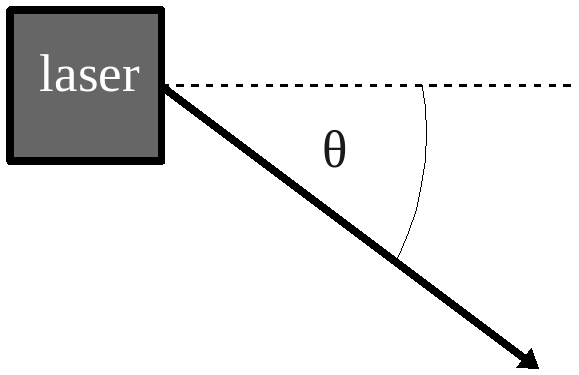
\includegraphics[width=0.8\linewidth]{./pics/coding/laserscanner2.png}
	\caption{How laser angles are referenced. In this diagram the laser is pointing to the right along the dotted line, the angle $\theta$ is the angle of a laser scan point, in this example $\theta$ is negative.}
	\label{fig:laserangles}
\end{figure} 

\begin{figure}
	\centering
	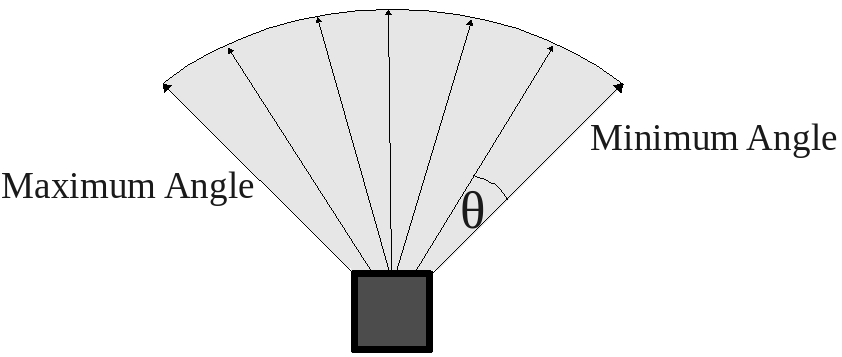
\includegraphics[width=\linewidth]{./pics/coding/laserscanner.png}
	\caption{A laser scanner. The minimum angle is the angle of the rightmost laser scan, the maximum angle is the leftmost laser scan. $\theta$ is the scan resolution of the laser, it is the angle between each laser scan, given in 0.01 degrees.}
	\label{fig:laserproxy}
\end{figure} 

\subsubsection{RangerProxy}
The RangerProxy is a proxy for more general ranging, it supports the sonar, laser and IR proxies. It has the same function as the SonarProxy in that you can use the code \verb\rangerProxy_name[ranger_number]\ to return the distance from ranger \verb\ranger_number\ to an obstacle. It also has many of the same functions as the LaserProxy, such as a minimum angle and a maximum angle and a scanning resolution, mostly these are for retrieving data about how the rangers are arranged or what size the ranging devices are. 

\subsubsection{BlobfinderProxy}
The blobfinder module analyses a camera image for areas of a desired colour and returns an array of the structure \verb\playerc_blobfinder_blob_t\, this is the structure used to store blob data. First we will cover how to get this data from the blobfinder proxy, then we will discuss the data stored in the structure.
\begin{itemize}
	\item \verb\GetCount\: Returns the number of blobs seen.
	\item \verb\blobProxy_name[blob_number]\: This returns the blob structure data for the blob with the index \verb\blob_number\. Blobs are sorted by index in the order that they appear in the image from left to right. This can also be achieved with the BlobfinderProxy function \verb\GetBlob(blob_number)\.
\end{itemize}

Once we receive the blob structure from the proxy we can extract data we need. The \verb\playerc_blobfinder_blob_t\ structure contains the following fields:
\begin{itemize}
	\item \verb\color\: The colour of the blob it detected. This is given as a hexadecimal value.
	\item \verb\area\: The area of the blob's bounding box.
	\item \verb\x\: The horizontal coordinate of the geometric centre of the blob's bounding box (see figure \ref{fig:blobimage}).
	\item \verb\y\: The vertical coordinate of the geometric centre of the blob's bounding box (see figure \ref{fig:blobimage}).
	\item \verb\left\: The horizontal coordinate of the left hand side of the blob's bounding box (see figure \ref{fig:blobimage}).
	\item \verb\right\: The horizontal coordinate of the right hand side of the blob's bounding box (see figure \ref{fig:blobimage}).
	\item \verb\top\: The vertical coordinate of the top side of the blob's bounding box (see figure \ref{fig:blobimage}).
	\item \verb\bottom\: The vertical coordinate of the bottom side of the blob's bounding box (see figure \ref{fig:blobimage}).
\end{itemize}

\begin{figure}
	\centering
	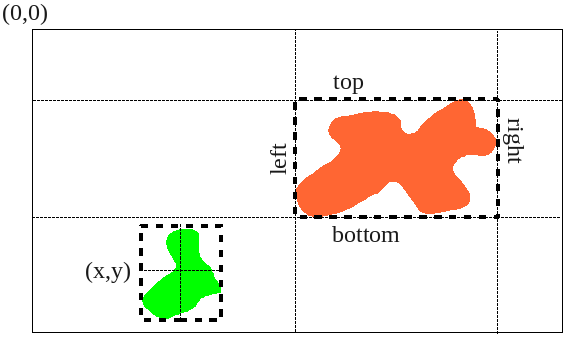
\includegraphics[width=\linewidth]{./pics/coding/blobfinder_image.png}
	\caption{What the fields in playerc\_blobfinder\_blob\_t mean. The blob on the left has a geometric centre at $(x,y)$, the blob on the right has a bounding box with the top left corner at $(left, top)$ pixels, and a lower right coordinate at $(right, bottom)$ pixels. Coordinates are given with reference to the top left corner of the image.}
	\label{fig:blobimage}
\end{figure} 

\subsubsection{GripperProxy}
The GripperProxy allows you to control the gripper, once the gripper is holding an item, the simulated robot will carry it around wherever it goes. Without a gripper you can only jostle an item in the simulation and you would have to manually tell the simulation what to do with an item. The GripperProxy can also tell you if an item is between the gripper teeth because the gripper model has inbuilt beams which can detect if they are broken. 
\begin{itemize}
	\item \verb\GetBeams\: This command will tell you if there is an item inside the gripper. If it is a value above 0 then there is an item to grab.
	\item \verb\GetState\: This will tell you whether the gripper is opened or closed. If the command returns a 1 then the gripper is open, if it returns 2 then the gripper is closed.
	\item \verb\Open\: Tells the gripper to open. This will cause any items that were being carried to be dropped.
	\item \verb\Close\: Tells the gripper to close. This will cause it to pick up anything between its teeth.
\end{itemize}


\subsubsection{SimulationProxy}
The simulation proxy allows your code to interact with and change aspects of the simulation, such as an item's pose or its colour. 
\paragraph{Get/Set Property}
To change a property of an item in the simulation we use the following function:
\newline\verb\SetProperty(char *item_name, char *property, void *value, size_t value_len)\
\begin{itemize}
	\item \verb\item_name\: this is the name that you gave to the object in the worldfile, it could be \emph{any} model that you have described in the worldfile. For example, in section \ref{sec:exampleRobot} in the worldfile we declared a Bigbob type robot which we called ``bob1'' so the \verb\item_name\ for that object is ``bob1''. Similarly in section \ref{sec:otherStuff} we built some models of oranges and called the ``orange1'' to ``orange4'' so the item name for one of these would be ``orange1''. Anything that is a model in your worldfile can be altered by this function, you just need to have named it, no drivers need to be declared in the configuration file for this to work either. We didn't write drivers for the oranges but we could still alter their properties this way.
	\item \verb\property\: There are only certain properties about a model that you can change. You specify which one you want with a string. Since the properties you can change are fixed then these strings are predefined (see stage.hh):
	\begin{itemize}
		\item \verb\"_mp_color"\: The colour of the item. 
		\item \verb\"_mp_watts"\: The number of watts the item needs.
		\item \verb\"_mp_mass"\: The mass of the item.
		\item \verb\"_mp_fiducial_return"\: sets whether the item is detectable to the fiducial finder on a robot.
		\item \verb\"_mp_laser_return"\: sets whether the item is detectable to the laser on a robot.
		\item \verb\"_mp_obstacle_return"\: sets whether the robot can collide with the item.
		\item \verb\"_mp_ranger_return"\: sets whether the item is detectable to the rangers on a robot.
		\item \verb\"_mp_gripper_return"\: sets whether the item can be gripped by a gripper or jostled by the robot colliding with it.
	\end{itemize}
	\item \verb\value\: The value you want to assign to the property. For the return parameters this can simply be a 0 or a 1, for the watts and mass it can be a numerical value. For the colour of the item this is a \verb\uint32_t\ 8 digit long hexadecimal number. The first 2 digits are the alpha value of the colour, the second two are its red value, the next two are its green value and the final two are the blue colour value. So red, for instance, would be  uint32\_t red = 0xffff0000, green would be 0xff00ff00 and blue is 0xff0000ff. A nice shade of yellow might be 0xffffcc11.
	\item \verb\value_len\: is the size of the value you gave in bytes. This can easily be found with the C or C++ \verb\sizeof()\ operator.
\end{itemize}
Similarly the following function can be used to get property information:\newline
\verb\GetProperty(char *item_name, char *property, void *value, size_t value_len)\
Instead of setting the given property of the item, this will write it to the memory block pointed to by \verb\*value\.

\paragraph{Get/Set Pose}
The item's pose is a special case of the Get/SetProperty function, because it is likely that someone would want to move an item in the world they created a special function to do it.\newline
\verb\SetPose2d(char *item_name, double x, double y, double yaw)\\newline
In this case \verb\item_name\ is as with Get/SetProperty, but we can directly specify its new coordinates and yaw (coordinates and yaws are given with reference to the map's origin).\newline
\verb\GetPose2d(char *item_name, double &x, double &y, double &yaw)\\newline
This is like SetPose2d only this time it writes the coordinates and yaw to the given addresses in memory.

\subsubsection{General Useful Commands}

\paragraph{Read()}
To make the proxies update with new sensor data we need to tell the player server to update, we can do this using the PlayerClient object which we used to connect to the server. All we have to do is run the command \verb\playerClient_name.Read()\ every time the data needs updating (where playerClient\_name is the name you gave the PlayerClient object). Until this command is run, the proxies and any sensor information from them will be empty. 
The devices on a typical robot are asynchronous and the devices in a \plst simulation are also asynchronous, so running the \verb\Read()\ command won't always update everything at the same time, so it may take several calls before some large data structures (such as a camera image) gets updated.

\paragraph{GetGeom()}
Most of the proxies have a function called \verb\GetGeom\ or \verb\GetGeometry\ or \verb\RequestGeometry\, or words to that effect. What these functions do is tell the proxy retrieve information about the device, usually its size and pose (relative to the robot). The proxies don't know this by default since this information is specific to the robot or the \plst robot model. If your code needs to know this kind of information about a device then the proxy must run this command first.


\subsection{Using Proxies: A Case Study}

To demonstrate how to write code to control a \pl device or \plst simulation we will use the example robot ``Bigbob'' developed in sections \ref{sec:buildingRobot} and \ref{sec:WritingConfigurationFile} which collects oranges and juice cartons from a factory floor. In previous sections we have developed the Stage model for this robot and its environment and the configuration file to control it. Now we can begin to put everything together to create a working simulation of this robot.

\subsubsection{The Control Architecture}
To collect rubbish we have three basic behaviours: 
\begin{itemize}
	\item Wandering: to search for rubbish. 
	\item Moving towards item: for when an item is spotted and the robot wants to collect it
	\item Collecting item: for dealing with collecting items.
\end{itemize}
The robot will also avoid obstacles but once this is done it will switch back to its previous behaviour. The control will follow the state transitions shown in figure \ref{fig:archstructure}.

\begin{figure}
	\centering
	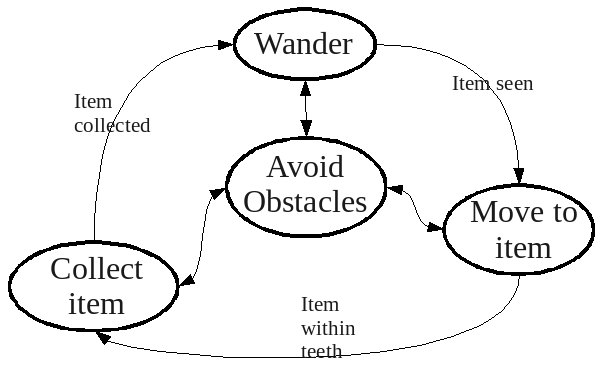
\includegraphics[width=\linewidth]{./pics/coding/arch_structureOA.png}
	\caption{The state transitions that the Bigbob rubbish collecting robot will follow.}
	\label{fig:archstructure}
\end{figure} 

\subsubsection{Beginning the Code}

In section \ref{sec:exampleconnectingtoserver} we discussed how to connect to the \pl server and proxies attached to the server, and developed the following code:
\begin{verbatim}
#include <stdio.h>
#include <libplayerc++/playerc++.h>

int main(int argc, char *argv[])
{
      /*need to do this line in c++ only*/
      using namespace PlayerCc;
	
      PlayerClient    robot("localhost");

      Position2dProxy p2dProxy(&robot,0);
      SonarProxy      sonarProxy(&robot,0);
      BlobfinderProxy blobProxy(&robot,0);
      LaserProxy      laserProxy(&robot,0);

      //some control code
      return 0;
}
\end{verbatim}
Using our knowledge of the proxies discussed in section \ref{sec:interactingwithproxies} we can build controlling code on top of this basic code. 
Firstly, it is good practice to enable the motors and request the geometry for all the proxies. This means that the robot will move and that if we need to know about the sensing devices the proxies will have that information available.
\begin{verbatim}
//enable motors
p2dProxy.SetMotorEnable(1);

//request geometries
p2dProxy.RequestGeom();
sonarProxy.RequestGeom();
laserProxy.RequestGeom();
//blobfinder doesn't have geometry
\end{verbatim}
Once things are initialised we can enter the main control loop. At this point we should tell the robot to read in data from its devices to the proxies.
\begin{verbatim}
while(true)
{
      robot.Read();

      //control code
}
\end{verbatim}

\subsubsection{Wander}

first we will initialise a couple of variables which will be the forward speed and the turning speed of the robot, we'll put this with the proxy initialisations.
\begin{verbatim}
Position2dProxy p2dProxy(&robot,0);
SonarProxy      sonarProxy(&robot,0);
BlobfinderProxy blobProxy(&robot,0);
LaserProxy      laserProxy(&robot,0);

double forwardSpeed, turnSpeed;
\end{verbatim}

Let's say that Bigbob's maximum speed is 1 metre/second and it can turn 90$^\circ$ a second. We will write a small subfunction to randomly assign forward and turning speeds between 0 and the maximum speeds.
\begin{verbatim}
void Wander(double *forwardSpeed, double *turnSpeed)
{
      int maxSpeed = 1;
      int maxTurn = 90;
      double fspeed, tspeed;
	
      //fspeed is between 0 and 10
      fspeed = rand()%11;
      //(fspeed/10) is between 0 and 1
      fspeed = (fspeed/10)*maxSpeed;
	
      tspeed = rand()%(2*maxTurn);
      tspeed = tspeed-maxTurn;
      //tspeed is between -maxTurn and +maxTurn
	
      *forwardSpeed = fspeed;
      *turnSpeed = tspeed;
} 
\end{verbatim}
In the control loop we include a call to this function and then set the resulting speeds to the motors.
\begin{verbatim}
while(true)
{		
      // read from the proxies
      robot.Read();

      //wander
      Wander(&forwardSpeed, &turnSpeed);

      //set motors
      p2dProxy.SetSpeed(forwardSpeed, dtor(turnSpeed));
}
\end{verbatim}

At present the motors are being updated every time this control loop executes, and this leads to some erratic behaviour from the robot. Using the \verb\sleep()\\footnote{sleep() is a standard C function and is included in the unistd.h header.} command we will tell the control loop to wait one second between each execution. At this point we should also seed the random number generator with the current time so that the wander behaviour isn't exactly the same each time. For the sleep command we will need to include \verb\unistd.h\ and to seed the random number generator with the current system time we will need to include \verb\time.h\.
\begin{verbatim}
#include <stdio.h>
#include <unistd.h>
#include <time.h>
#include <libplayerc++/playerc++.h>

void Wander(double *forwardSpeed, double *turnSpeed)
{
      //wander code...
} 

int main(int argc, char *argv[])
{	
      /*need to do this line in c++ only*/
      using namespace PlayerCc;

      //connect to proxies
      double forwardSpeed, turnSpeed;
	
      srand(time(NULL));
	
      //enable motors
      //request geometries
	
      while(true)
      {		
            // read from the proxies
            robot.Read();

            //wander
            Wander(&forwardSpeed, &turnSpeed);
		
            //set motors
            p2dProxy.SetSpeed(forwardSpeed, dtor(turnSpeed));
            sleep(1);
      }
}
\end{verbatim}

\subsubsection{Obstacle Avoidance}
Now we need to write a subfunction that checks the sonars for any obstacles and amends the motor speeds accordingly.
\begin{verbatim}
void AvoidObstacles(double *forwardSpeed, double *turnSpeed, \
      SonarProxy &sp)
{
      //will avoid obstacles closer than 40cm
      double avoidDistance = 0.4;
      //will turn away at 60 degrees/sec
      int avoidTurnSpeed = 60;
      
      //left corner is sonar no. 2
      //right corner is sonar no. 3
      if(sp[2] < avoidDistance)
      {
            *forwardSpeed = 0;
            //turn right
            *turnSpeed = (-1)*avoidTurnSpeed;
            return;
      }
      else if(sp[3] < avoidDistance)
      {
            *forwardSpeed = 0;
            //turn left
            *turnSpeed = avoidTurnSpeed;
            return;
      }
      else if( (sp[0] < avoidDistance) && \
               (sp[1] < avoidDistance))
      {
            //back off a little bit
            *forwardSpeed = -0.2;
            *turnSpeed = avoidTurnSpeed;  
            return;
      }
      
      return; //do nothing
}
\end{verbatim}
This is a very basic obstacle avoidance subfunction will update the motor speeds only if there is an obstacle to avoid. If we call this function just before sending data to the motors then it will overwrite any other behaviours so that the obstacle will be avoided. Once the obstacle is no longer in the way then the robot will continue as it was, this will allow us to transition from any behaviour into obstacle avoidance and then back again, as per the requirement of our control structure. All we need to do now is call this function in our control loop:
\begin{verbatim}
while(true)
{		
    // read from the proxies
    robot.Read();
		
    //wander
    Wander(&forwardSpeed, &turnSpeed);
		
    //avoid obstacles
    AvoidObstacles(&forwardSpeed, &turnSpeed, sonarProxy);
		
    //set motors
    p2dProxy.SetSpeed(forwardSpeed, dtor(turnSpeed));
    sleep(1);
}
\end{verbatim}

\subsubsection{Move To Item}
For this state we want the robot to move towards a blob that it has spotted. There may be several blobs in its view at once, so we'll tell the robot to move to the largest one because it's probably the closest to the robot. The following subfunction finds the largest blob and turns the robot so that the blob's centre is near the centre of the image. The robot will then move towards the blob.
\begin{verbatim}
void MoveToItem(double *forwardSpeed, double *turnSpeed, \
      BlobfinderProxy &bfp)
{
      int i, centre;
      int noBlobs = bfp.GetCount();
      playerc_blobfinder_blob_t blob;
      int turningSpeed = 10;
      
      /*number of pixels away from the image centre a blob
      can be to be in front of the robot*/
      int margin = 10;
      
      int biggestBlobArea = 0;
      int biggestBlob = 0;
      
      //find the largest blob
      for(i=0; i<noBlobs; i++)
      {
            //get blob from proxy
            playerc_blobfinder_blob_t currBlob = bfp[i];
            
            if(currBlob.area > biggestBlobArea)
            {
                  biggestBlob = i;
                  biggestBlobArea = currBlob.area;
            }
      }
      blob = bfp[biggestBlob];
            
      // find centre of image
      centre = bfp.GetWidth()/2;
      
      //adjust turn to centre the blob in image
      /*if the blob's centre is within some margin of the image 
      centre then move forwards, otherwise turn so that it is 
      centred. */
      //blob to the left of centre
      if(blob.x < centre-margin)
      {
            *forwardSpeed = 0;
            //turn left
            *turnSpeed = turningSpeed;
      }
      //blob to the right of centre
      else if(blob.x > centre+margin)
      {
            *forwardSpeed = 0;
            //turn right
            *turnSpeed = -turningSpeed;
      }
      //otherwise go straight ahead
      else
      {
            *forwardSpeed = 0.5;
            *turnSpeed = 0;      
      }
      
      return;
}
\end{verbatim}

We want the robot to transition to this state whenever an item is seen, so we put a conditional statement in our control loop like so:
\begin{verbatim}
if(blobProxy.GetCount() == 0)
{
      //wander
      Wander(&forwardSpeed, &turnSpeed);
}
else
{
      //move towards the item
      MoveToItem(&forwardSpeed, &turnSpeed, blobProxy);
}
\end{verbatim}

\subsubsection{Collect Item}
This behaviour will be the most difficult to code because Stage doesn't support pushable objects (the required physics is far too complex), what happens instead is that the robot runs over the object and just jostles it a bit. 
As a work-around to this problem we will have to somehow find out which item is between Bigbob's teeth so that we can find its ``name'' and then change that item's pose (for which we need the item's name) so that it is no longer in the simulation. In essence, instead of having our robot eat rubbish and store it within its body, what we are doing is making the laser zap the rubbish out of existence.

We can find the name of an item between Bigbob's teeth by cross referencing the robot's pose with the locations of the items in the world to find out which item is nearest the robot's laser. The first step is to create a list of all the items in the world, their names and their poses at initialisation. Since we know the names of the items are ``orange1'' to ``orange4'' and ``carton1'' to ``carton4'', we can find their poses with a simple call to a simulation proxy. We'll have to connect to the simulation proxy with our code first using the line \verb\SimulationProxy simProxy(&robot,0);\, then we can access this information and put it into a struct.
\begin{verbatim}
struct Item
{
      char name[16];
      double x;
      double y;
}typedef item_t;
\end{verbatim}
We can populate the structure with information using the following code:
\begin{verbatim}
item_t itemList[8];

void RefreshItemList(item_t *itemList, SimulationProxy &simProxy)
{
      int i;
      	
      //get the poses of the oranges
      for(i=0;i<4;i++)
      {
            char orangeStr[] = "orange%d";
            sprintf(itemList[i].name, orangeStr, i+1);
            double dummy;  //dummy variable, don't need yaws.
            simProxy.GetPose2d(itemList[i].name, \
                  itemList[i].x, itemList[i].y, dummy);
      }
      	
      //get the poses of the cartons
      for(i=4;i<8;i++)
      {
            char cartonStr[] = "carton%d";
            sprintf(itemList[i].name, cartonStr, i-3);
            double dummy;  //dummy variable, don't need yaws.
            simProxy.GetPose2d(itemList[i].name, \
                  itemList[i].x, itemList[i].y, dummy);
      }
      
      return;
}
\end{verbatim}
Where \verb\itemList\ is an \verb\item_t\ array of length 8. 

Next we can begin the ``Collect Item'' behaviour, which will be triggered by something breaking the laser beam. When this happens we will check the area around Bigbob's teeth, as indicated by figure \ref{fig:bigboblaserradius}. We know the distance from the centre of this search circle to Bigbob's origin (0.625m) and the radius of the search circle (0.375m), we can get the robot's exact pose with the following code.
\begin{verbatim}
double x, y, yaw;
simProxy.GetPose2d("bob1", x, y, yaw);
\end{verbatim}
Cross referencing the robot's position with the item positions is a matter of trigonometry, we won't reproduce the code here, but the full and final code developed for the Bigbob rubbish collecting robot is included in appendix D. The method we used is to find the Euclidian distance of the items to the circle centre, and the smallest distance is the item we want to destroy. We made a subfunction called \verb\FindItem\ that returns the index of the item to be destroyed.

\begin{figure}
	\centering
	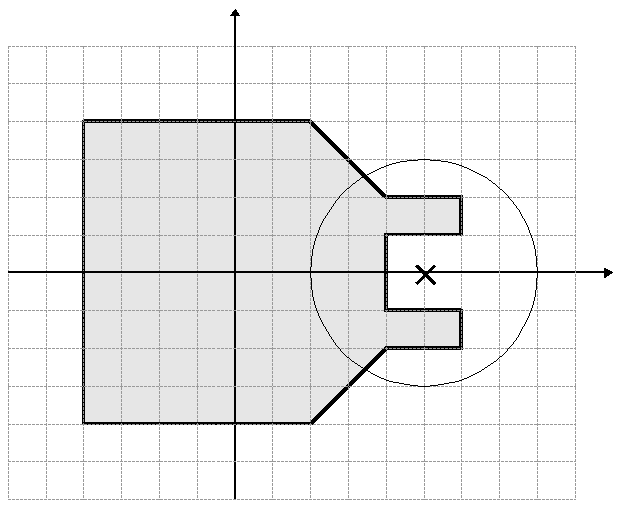
\includegraphics[width=0.7\linewidth]{./pics/coding/bigbob_radius.png}
	\caption{Where to look for items which may have passed through Bigbob's laser.}
	\label{fig:bigboblaserradius}
\end{figure} 

Now that we can find the item to destroy it's fairly simple to trigger our subfunction when the laser is broken so we can find and destroy an item.
\begin{verbatim}
if(laserProxy[90] < 0.25)
{
      int destroyThis;

      /*first param is the list of items in the world
      second is length of this list
      third parameter is the simulation proxy with 
      the pose information in it*/
      destroyThis = FindItem(itemList, 8, simProxy);
 
      //move it out of the simulation
      simProxy.SetPose2d(itemList[destroyThis].name, -10, -10, 0);
      RefreshItemList(itemList, simProxy);
}
\end{verbatim}
The laser has 180 points, so point number 90 is the one which is perpendicular to Bigbob's teeth. This point returns a maximum of 0.25, so if its range was to fall below this then something has passed through the laser beam. We then find the item closest to the robot's teeth and move that item to coordinate $(-10, -10)$ so it is no longer visible or accessible.
\newline
Finally we have a working simulation of a rubbish collecting robot! The full code listing is included in appendix D, the simulation world and configuration files are in appendices B and C respectively.

\subsection{Simulating Multiple Robots}
Our robot simulation case study only shows how to simulate a single robot in a \plst environment. It's highly likely that a simulation might want more than one robot in it. In this situation you will need to build a model of every robot you need in the worldfile, and then its associated driver in the configuration file. Let's take a look at our worldfile for the case study, we'll add a new model of a new Bigbob robot called ``bob2'':
\begin{verbatim}
bigbob
(
	name "bob1"
	pose [-5 -6 45]
	color "green"
)

bigbob
(
	name "bob2"
	pose [5 6 225]
	color "yellow"
)
\end{verbatim}
If there are multiple robots in the simulation, the standard practice is to put each robot on its own port (see section \ref{sec:deviceAddress}). To implement this in the configuration file we need to tell \pl which port to find our second robot on:
\begin{verbatim}
driver( name "stage" 
        provides ["6665:position2d:0" "6665:sonar:0" 
        "6665:blobfinder:0" "6665:laser:0"] 
        model "bob1" )

driver( name "stage" 
        provides ["6666:position2d:0" "6666:sonar:0" 
        "6666:blobfinder:0" "6666:laser:0"] 
        model "bob2" )
\end{verbatim}
If you plan on simulating a large number of robots then it is probably worth writing a script to generate the world and configuration files.

When \plst is started, the \pl server automatically connects to all the used ports in your simulation and you control the robots separately with different PlayerClient objects in your code. For instance:
\begin{verbatim}
//first robot
PlayerClient robot1("localhost", 6665);
Position2dProxy p2dprox1(&robot1,0);
SonarProxy sprox1(&robot1,0);

//second robot
PlayerClient robot2("localhost", 6666);
Position2dProxy p2dprox2(&robot2,0);
SonarProxy sprox2(&robot2,0);
\end{verbatim}
Each \pl Client represents a robot, this is why when you connect to a proxy the PlayerClient is a constructor parameter. Each robot has a proxy for each of its devices, no robots share a proxy, so it is important that your code connects to every proxy of every robot in order to read the sensor information.
How you handle the extra PlayerClients and proxies is dependent on the scale of the simulation and your own personal coding preferences. It's a good idea, if there's more than maybe 2 robots in the simulation, to make a robot class which deals with connecting to proxies and the server, and processes all the information internally to control the robot. Then you can create an instance of this class for each simulated robot\footnote{obviously the robot's port number would need to be a parameter otherwise they'll all connect to the same port and consequently the same robot.} and all the simulated robots will run the same code.

An alternative to using a port for each robot is to use the same port but a different index. This will only work if the robots are all the same (or at least use the same interfaces, although different robots could be run on a different ports) and the robots only use one index for each of its devices. For example, the Bigbob robot uses interfaces and indexes: position2d:0, sonar:0, blobfinder:0 and laser:0 so it never uses more than one index. If we configured two Bigbob robots to use the same port but a different index our configuration file would be like this:
\begin{verbatim}
driver( name "stage" 
        provides ["6665:position2d:0" "6665:sonar:0" 
        "6665:blobfinder:0" "6665:laser:0"] 
        model "bob1" )

driver( name "stage" 
        provides ["6665:position2d:1" "6665:sonar:1" 
        "6665:blobfinder:1" "6665:laser:1"] 
        model "bob2" )
\end{verbatim}
In our code we could then establish the proxies using only one PlayerClient:
\begin{verbatim}
PlayerClient robot("localhost", 6665);

//first robot
Position2dProxy p2dprox1(&robot,0);
SonarProxy sprox1(&robot,0);

//second robot
Position2dProxy p2dprox2(&robot,1);
SonarProxy sprox2(&robot,1);

//shared Simultion proxy...
SimulationProxy sim(&robot,0);
\end{verbatim}
The main advantage of configuring the robot swarm this way is that it allows us to only have one simulation proxy which is shared by all robots. This is good since there is only ever one simulation window that you can interact with and so multiple simulation proxies are unnecessary.

\section{Useful Links}

\begin{itemize}

\item Player 2.1.0 Manual \\
\url{http://playerstage.sourceforge.net/doc/Player-2.1.0/player/}

\item Stage 3.0.1 Manual \\
\url{http://playerstage.sourceforge.net/doc/stage-3.0.1/}

\item Stage 2.0.0 Manual\\
\url{http://playerstage.sourceforge.net/doc/Stage-2.0.0/}

\item All Player Proxies in C\\
\url{http://playerstage.sourceforge.net/doc/Player-2.1.0/player/group__playerc__proxies.html}

\item All Player Proxies in C++\\
\url{http://playerstage.sourceforge.net/doc/Player-2.1.0/player/namespacePlayerCc.html}

\item Interfaces used by Player\\
\url{http://playerstage.sourceforge.net/doc/Player-2.1.0/player/group__interfaces.html}
\end{itemize}

\bibliographystyle{plain}
\bibliography{manualrefs}






\section{Appendices}

\subsection*{Appendix A. General Stage Model of Bigbob}\label{app:Abigbob.inc}
\verbatiminput{./appendices/bigbob.inc}

\subsection*{Appendix B. Worldfile, Containing Robot and Items in World}\label{app:Brobotsjunkworld}
\verbatiminput{./appendices/robots_and_junk.world}

\subsection*{Appendix C. Configuration file for Bigbob World}\label{app:Cconfig}
\verbatiminput{./appendices/test1.cfg}

\subsection*{Appendix D. Controlling Code for Bigbob Robot Simulation}\label{app:Dbigbobcode}
\verbatiminput{./appendices/bigbob.cc}





\end{document}
